\documentclass[letterpaper,11pt]{article}
\usepackage{jheppub}
%Uncomment next line if AMS fonts required
\usepackage{amsfonts}
\usepackage{xspace}
\usepackage{doi}
\usepackage{graphicx}
\usepackage{subcaption}
\usepackage{float}
\usepackage{minted}

\newcommand{\pt}{\ensuremath{p_{\mathrm{T}}}\xspace}
\newcommand{\PZpr}{\ensuremath{\mathrm{Z}^{\prime}}\xspace} % Z'
\newcommand{\PW}{\ensuremath{\mathrm{W}}\xspace} % W
\newcommand{\PWpr}{\ensuremath{\mathrm{W}^{\prime}}\xspace} % W'
\newcommand{\PX}{\ensuremath{\mathrm{X}}\xspace} % X
\newcommand{\PY}{\ensuremath{\mathrm{Y}}\xspace} % Y
\newcommand{\Pq}{\ensuremath{\mathrm{q}}\xspace} % q

\newcommand{\TODO}[1]{\textcolor{red}{TODO: #1}}

\begin{document}

%%%%%%%%%%%%%%%%%%%%%%
\section*{Particle Graph Autoencoders}
Author(s): Steven Tsan, Javier Duarte \\ 
\textit{University of California San Diego, La Jolla, CA 92130, USA}\\
Jean-Roch Vlimant\\
\textit{California Institute of Technology, Pasadena, CA 91125, USA}\\
Maurizio Pierini\\
\textit{European Organization for Nuclear Research (CERN), CH-1211, Geneva 23, Switzerland}

%\noindent \textit{Please do not write an introduction to anomaly detection - we will have one introduction at the beginning.  Furthermore, please give your method a concise name - it is fine to say \textbf{Concise Name: Longer Name that is More Specific.}  The length limit is five pages of text (not included references), with fewer pages preferred, and at most one additional page of figures if needed.}

\subsection{Method}
\label{sec:method}

%\noindent \textit{Please introduce the motivation for your method (not anomaly detection in general), how it works, and how you have implemented it.  Please include details about how you trained your algorithms and how you picked your hyperparameters.}\\

We propose particle graph autoencoders (PGAEs) based on graph neural networks~\cite{Shlomi:2020gdn} for unsupervised detection of new physics in multijet final states at the LHC. 
By embedding particle jet showers as a graph, GNNs are able to exploit particle-particle relationships to efficiently encode and reconstruct particle-level information within jets.
We posit that this can improve the capacity of autoencoders to learn a compressed representation of a jet and consequently help identify anomalous beyond-the-standard-model (BSM) multijet signal events from LHC data.

%Autoencoders are unsupervised ML models composed of two parts: an encoder that maps an input to a compressed representation and a decoder that reconstructs the input image.
%Autoencoders will learn to accurately reconstruct data similar to what is seen during its training; however, anomalous signals rare or absent in the training data will not be accurately reconstructed by autoencoders.  
%By measuring how much data is lost during reconstruction, one can distinguish between outlier events and background,cutting down on the possible candidates for new physics in our data.
In our PGAE model, we represent each input jet as a graph in which each particle of the jet is a node, and each node has an edge connecting it to every other particle in the jet (i.e. a fully-connected particle graph).
When encoding and decoding, the graph structure of the data remains the same, but the nodes' features, initially the particle's four-momentum $(E, p_x, p_y, p_z)$, have their dimensionality reduced during the encoding phase.
We note the model can be expanded to consider additional particle-level information, such as particle type, electromagnetic charge, and pileup probability weight~\cite{Bertolini:2014bba}.
For the encoder and decoder, we use the edge convolution layer from Ref.~\cite{DGCNN}, which performs message passing along the edges and aggregation of messages at the nodes of the graphs.
A schematic of this is shown in Fig.~\ref{fig:gae}. 


\begin{figure}[htpb]
    \centering
    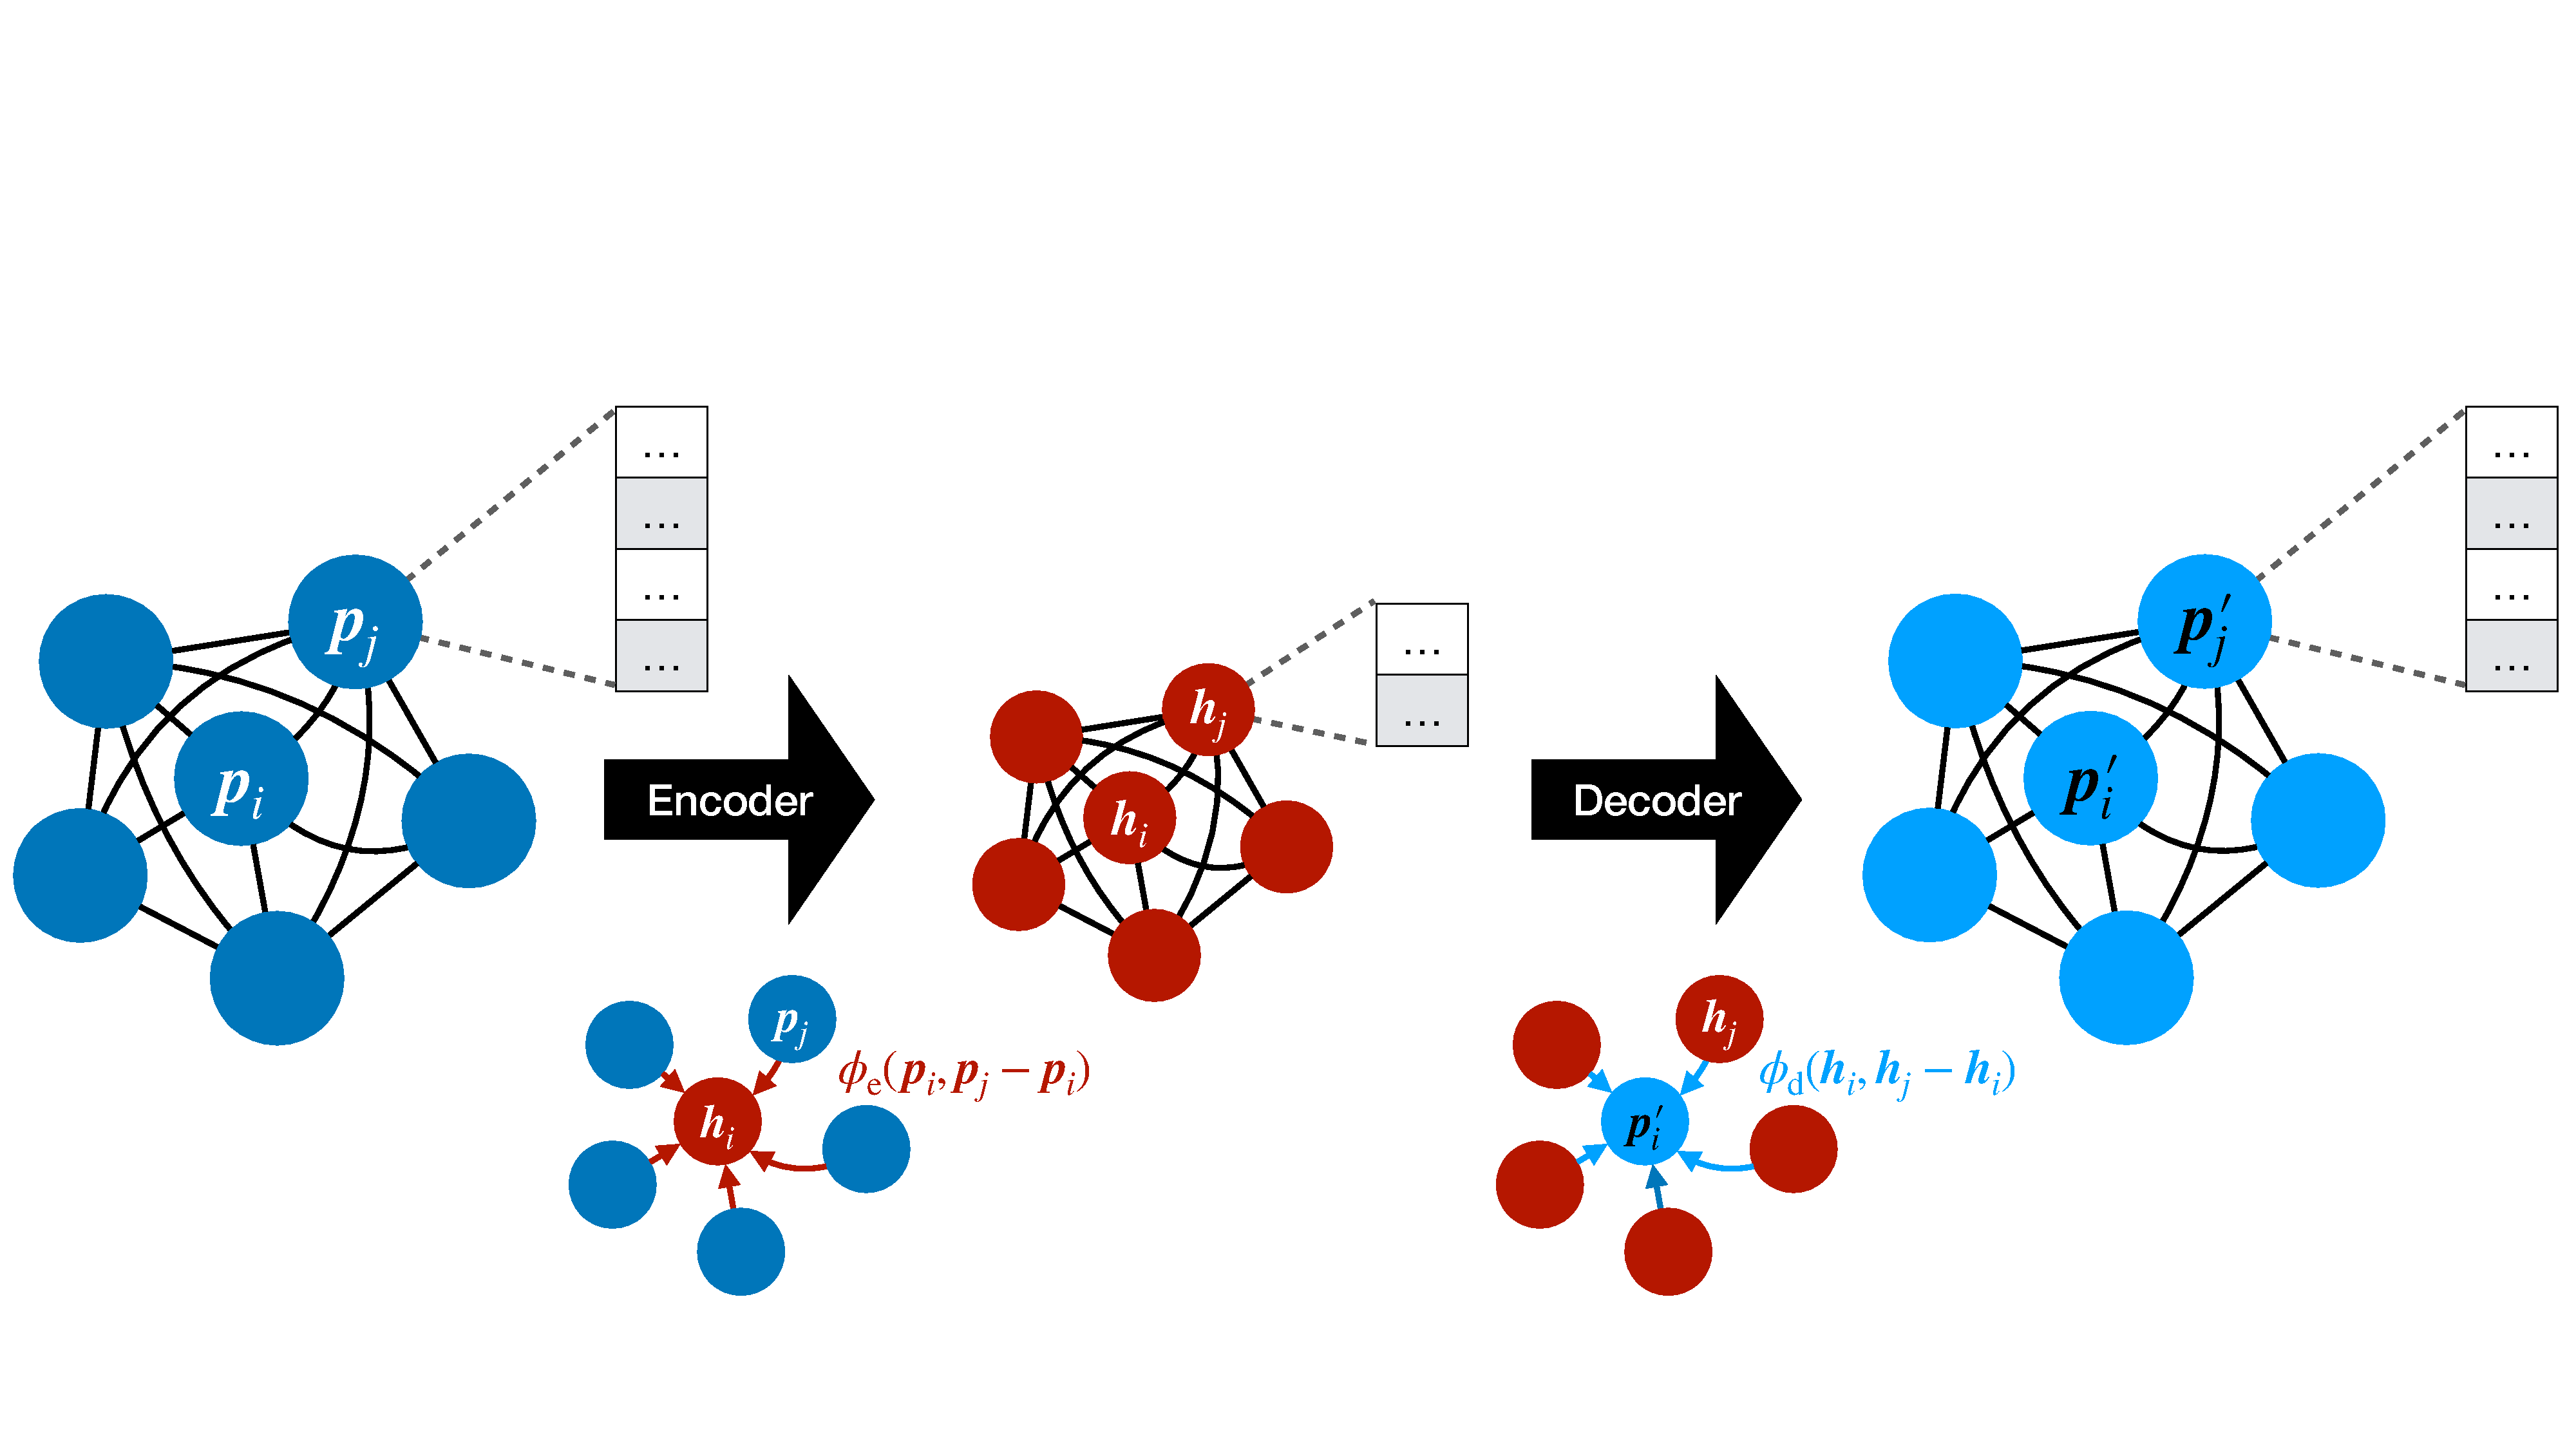
\includegraphics[width=\textwidth]{figures/GAE_new.pdf}
    \caption{Schematic of the particle graph autoencoder model proposed. 
    Each input jet is represented as a graph in which each particle of the jet is a node, and each node has an edge connecting it to every other particle in the jet.
    After an edge convolution layer~\cite{DGCNN}, each particle is encoded in a reduced two-dimensional latent space, before another edge convolution layer reconstructs each particle's four-momentum $(E, p_x, p_y, p_z)$.
}
    \label{fig:gae}
\end{figure}

% gnn architecture
The PGAE model is constructed using the PyTorch Geometric library~\cite{PyTorchGeometric}.
In this model, the input node features are first processed by a batch normalization layer~\cite{batchnorm}.
The encoder is an edge convolution layer~\cite{DGCNN}, built from a fully connected neural network $\phi_\mathrm{e}$ with layers of sizes $(8, 32, 32, 2)$ and rectified linear activation unit (ReLU) activation functions~\cite{relu}.
The first layer of dimension $8$ represents the input, which is given by $(\boldsymbol{p}_i, \boldsymbol{p}_j-\boldsymbol{p}_i)$, where $\boldsymbol{p}_i$ ($\boldsymbol{p}_j$) is the four-momentum for particle $i$ ($j$) and $i\neq j$.
The final layer produces a two-dimensional message vector from each pair of distinct particles.
These two-dimensional message vectors are aggregated (using a mean function) for each receiving particle
\begin{equation}
\boldsymbol{h}_i = \frac{1}{|\mathcal N(i)|}\sum_{j\in \mathcal N(i)} \phi_\mathrm{e}(\boldsymbol{p}_i, \boldsymbol{p}_j-\boldsymbol{p}_i)\,,
\end{equation}
where $\mathcal N(i)$ is the neighborhood of particles connected to the $i$th particle, which corresponds to all other particles in this case.
This summed message $\vec h_i$ is the bottleneck or encoded representation for the $i$th particle.
The decoder is also an edge convolution layer, containing a network $\phi_\mathrm{d}$ with layers of sizes $(4, 32, 32, 4)$ and ReLU activation functions, except for the final layer, which reconstructs each particle's momentum.
We note that the architecture itself is insensitive to the ordering of the input particles. 
PyTorch Geometric supports variable-size input graphs so there is no need for zero-padding.

% loss function and training
The model is trained with two different loss functions. 
The first is the mean squared error (MSE) between the input and output particles. 
This choice of loss function violates the permutation invariance of the algorithm because the particles must be reconstructed in the same order as they are input to achieve a small value of the loss function.
For this reason, we also investigate a second, alternative loss function, the nearest neighbor distance $D^\mathrm{NN}$, whose value does not depend on either the order of the input particles or the reconstructed particles~\cite{sparsegen_vae}.
Given two input sets of particles $\mathcal{M}$ and $\mathcal{N}$, expressed in terms of the momentum vectors $\boldsymbol{p}_i$ and $\boldsymbol{p}_j$ (with $i \in \mathcal{M}$ and $j \in \mathcal{N}$), the loss function is defined as
\begin{equation}
D^\mathrm{NN}(\mathcal{M}, \mathcal{N}) =  \frac{1}{|\mathcal{M}|}\sum_{i \in \mathcal{M}} \min_{j \in \mathcal{N}} \left(||\boldsymbol{p}_i - \boldsymbol{p}_j||\right)^2 + \frac{1}{|\mathcal{N}|}\sum_{j \in \mathcal{N}} \min_{i \in \mathcal{M}} \left(||\boldsymbol{p}_i - \boldsymbol{p}_j||\right)^2\,,
\label{eq:L_NND}
\end{equation}
where $||\boldsymbol{p}_i-\boldsymbol{p}_j||$ is the Euclidean distance.

\begin{figure}[htpb]
\centering
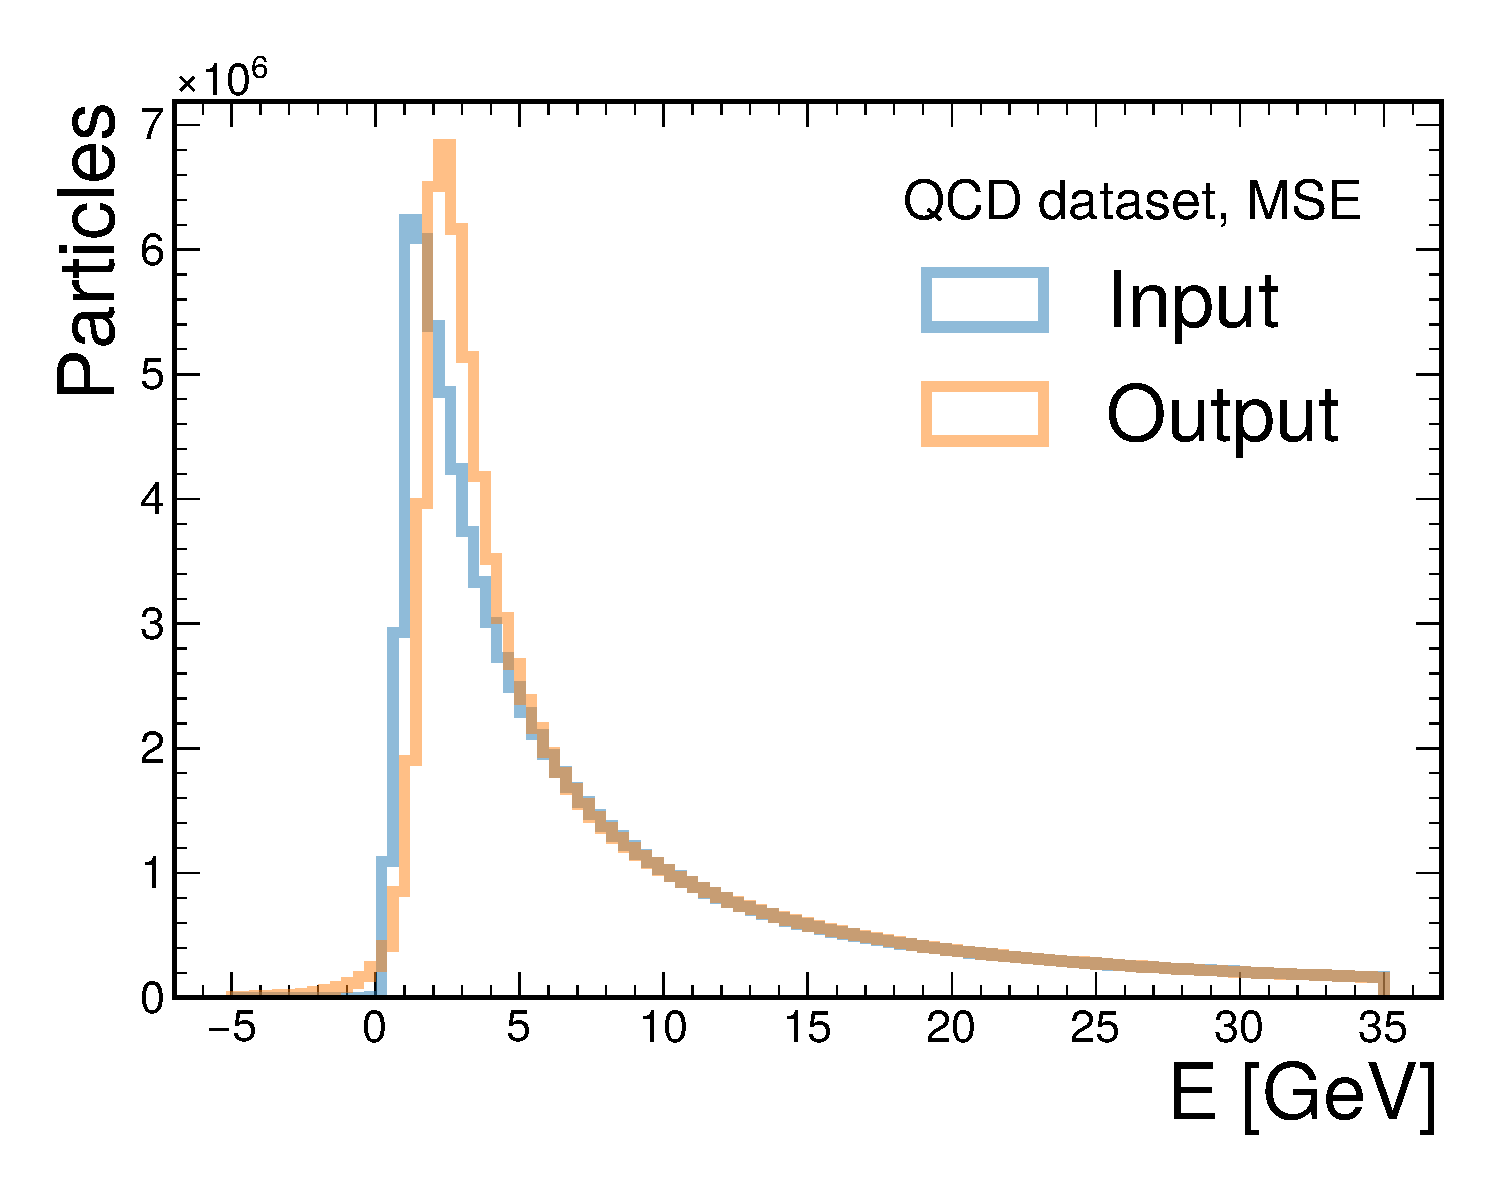
\includegraphics[width=0.24\textwidth]{figures/gae_mse/GNN_AE_EdgeConv_$E$.pdf}
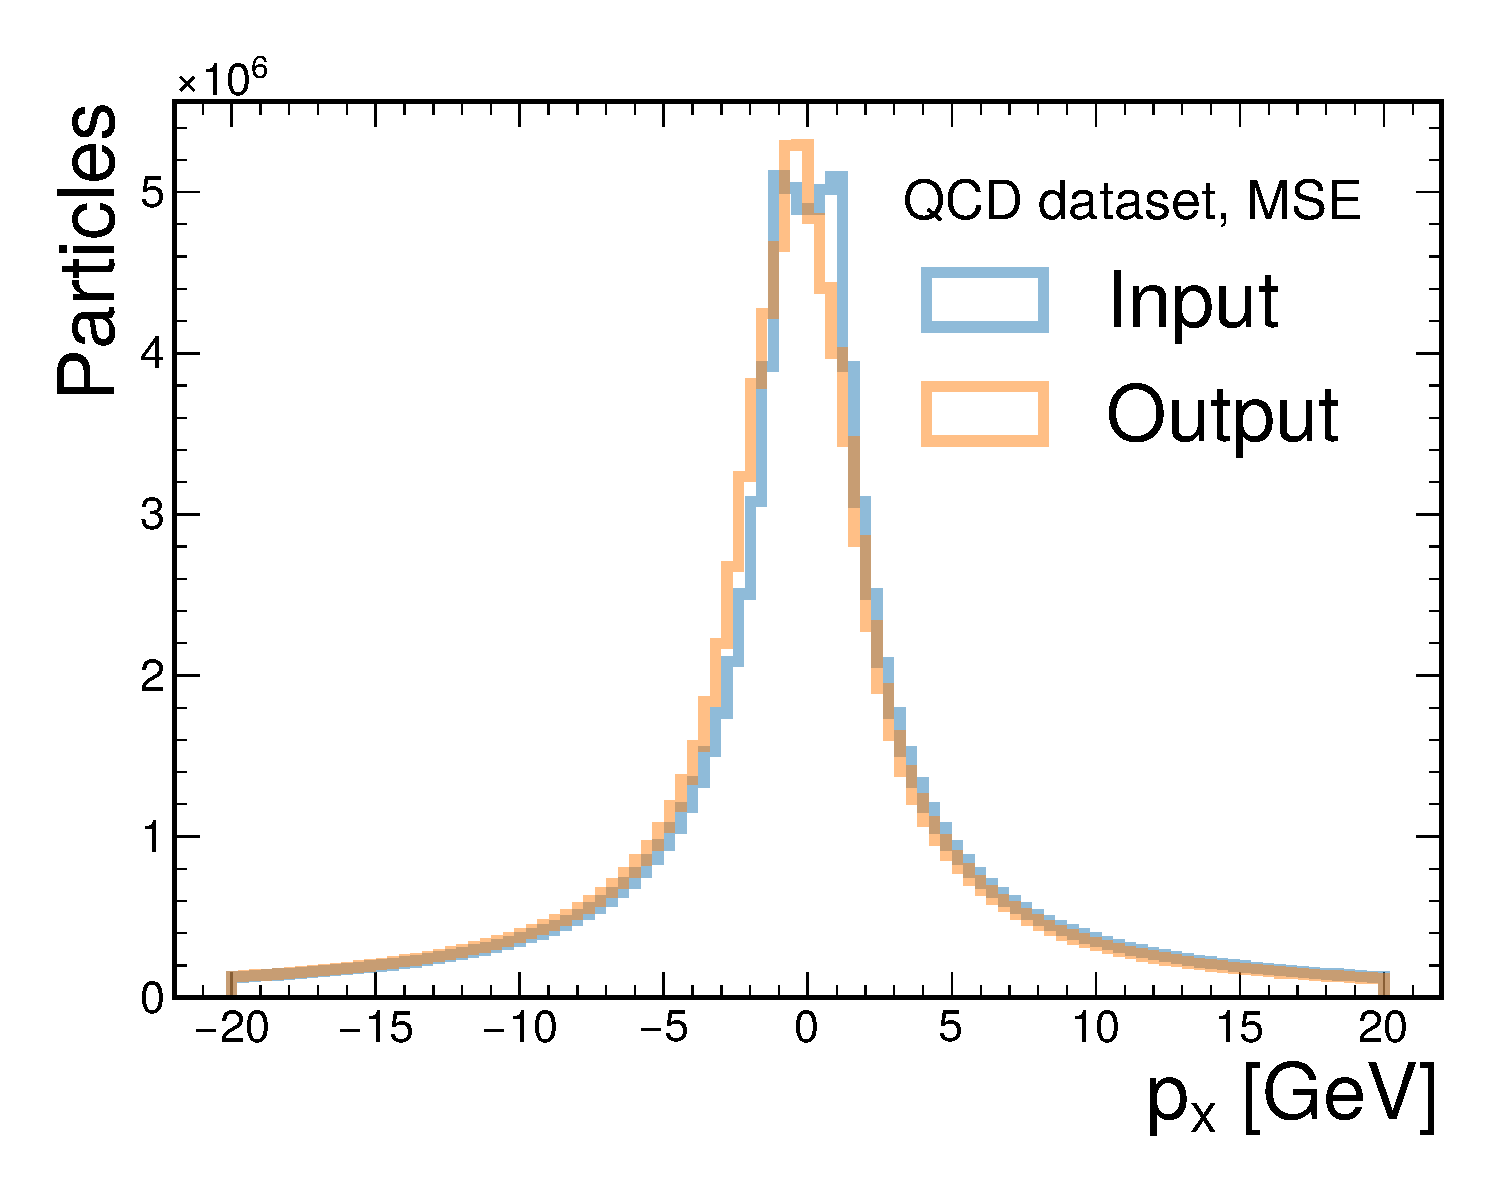
\includegraphics[width=0.24\textwidth]{figures/gae_mse/GNN_AE_EdgeConv_$p_x$.pdf}
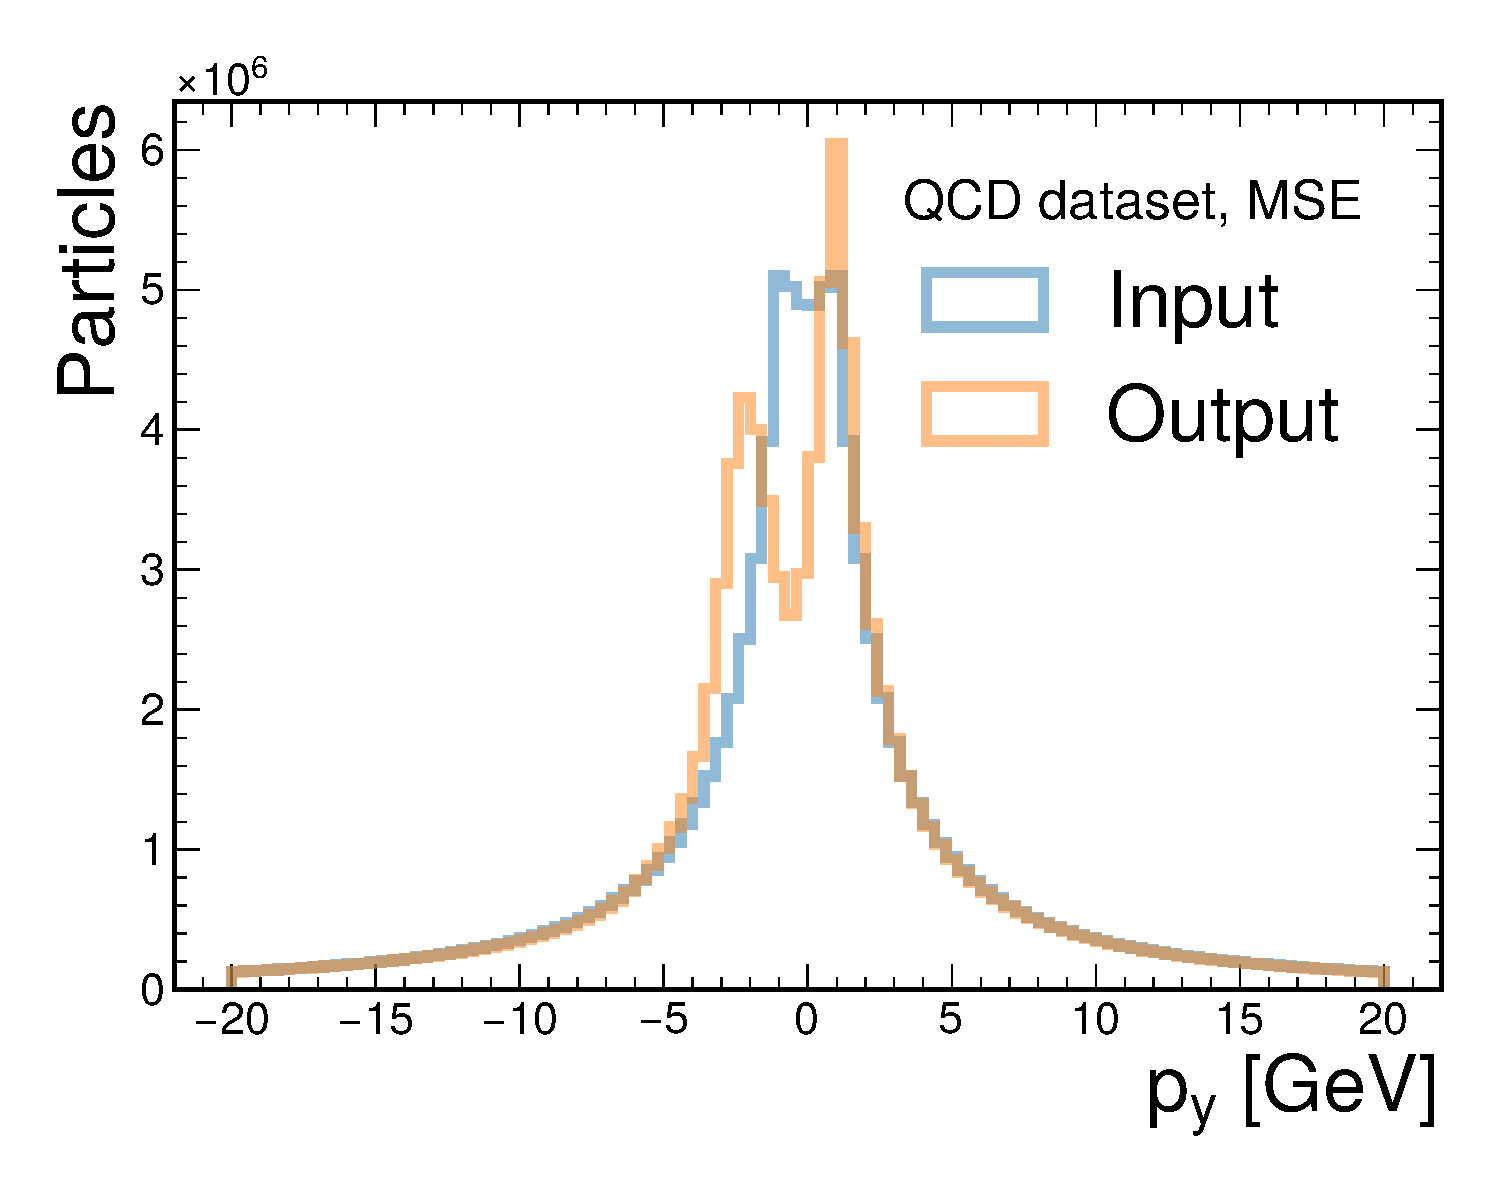
\includegraphics[width=0.24\textwidth]{figures/gae_mse/GNN_AE_EdgeConv_$p_y$.pdf}
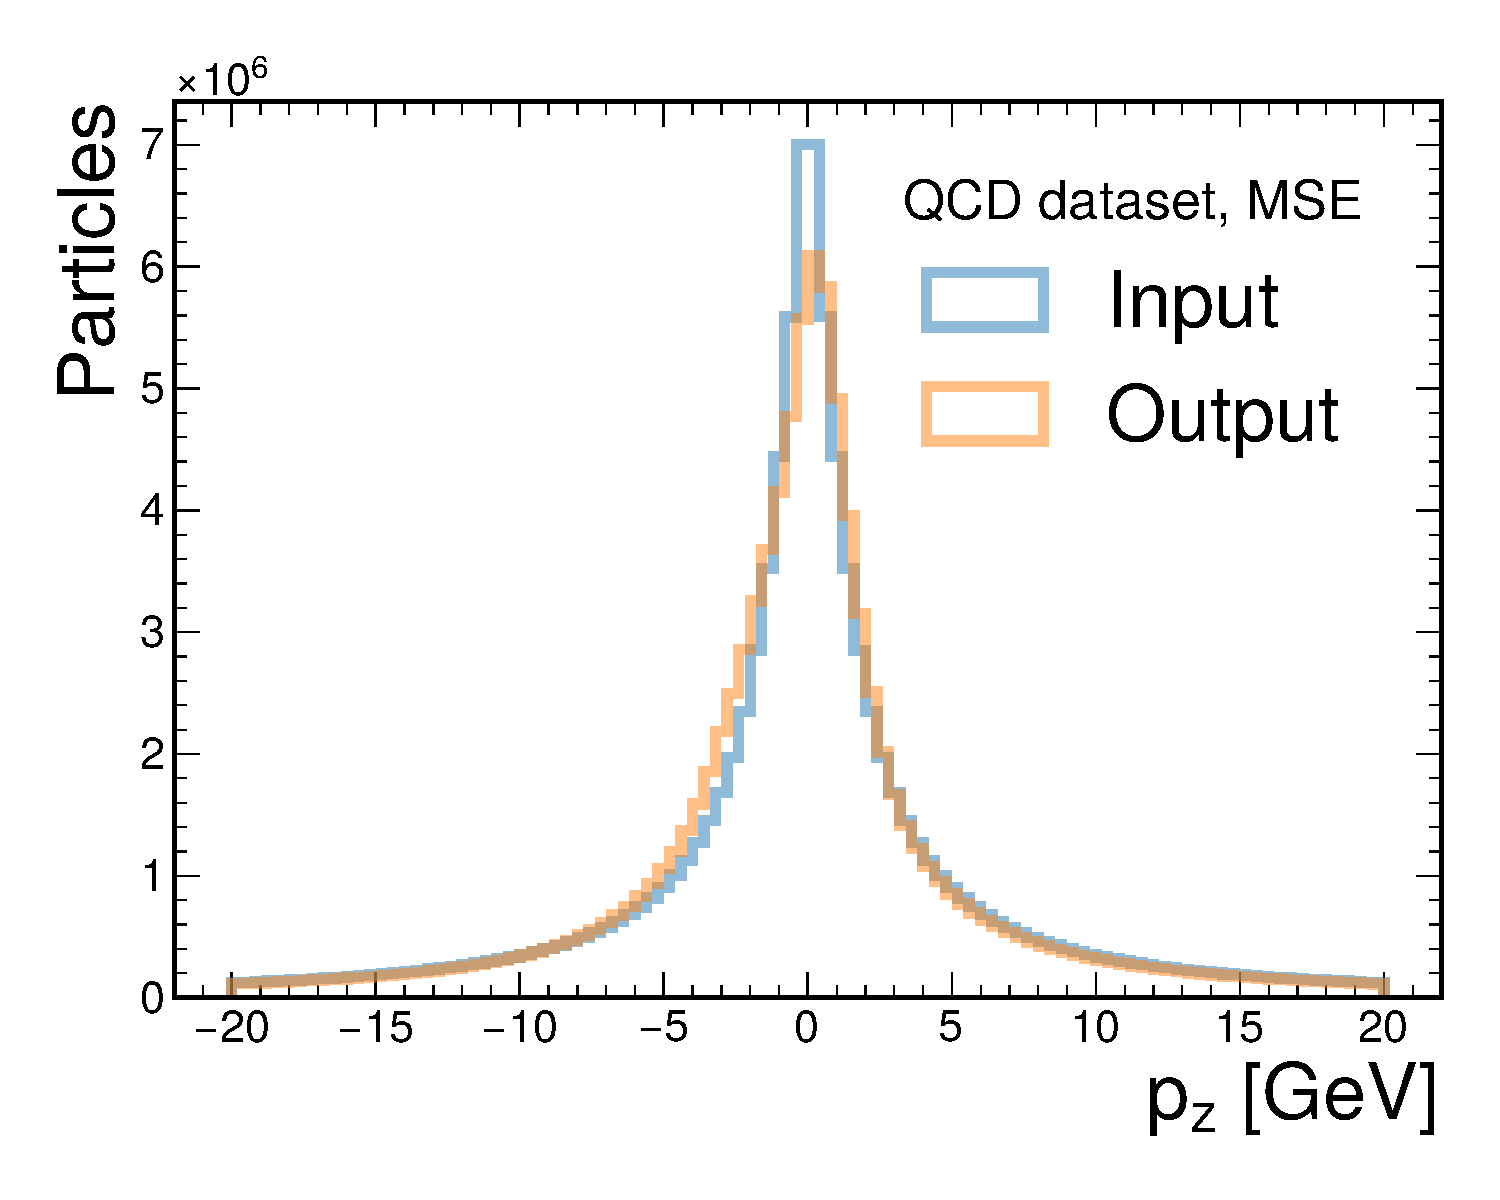
\includegraphics[width=0.24\textwidth]{figures/gae_mse/GNN_AE_EdgeConv_$p_z$.pdf}\\
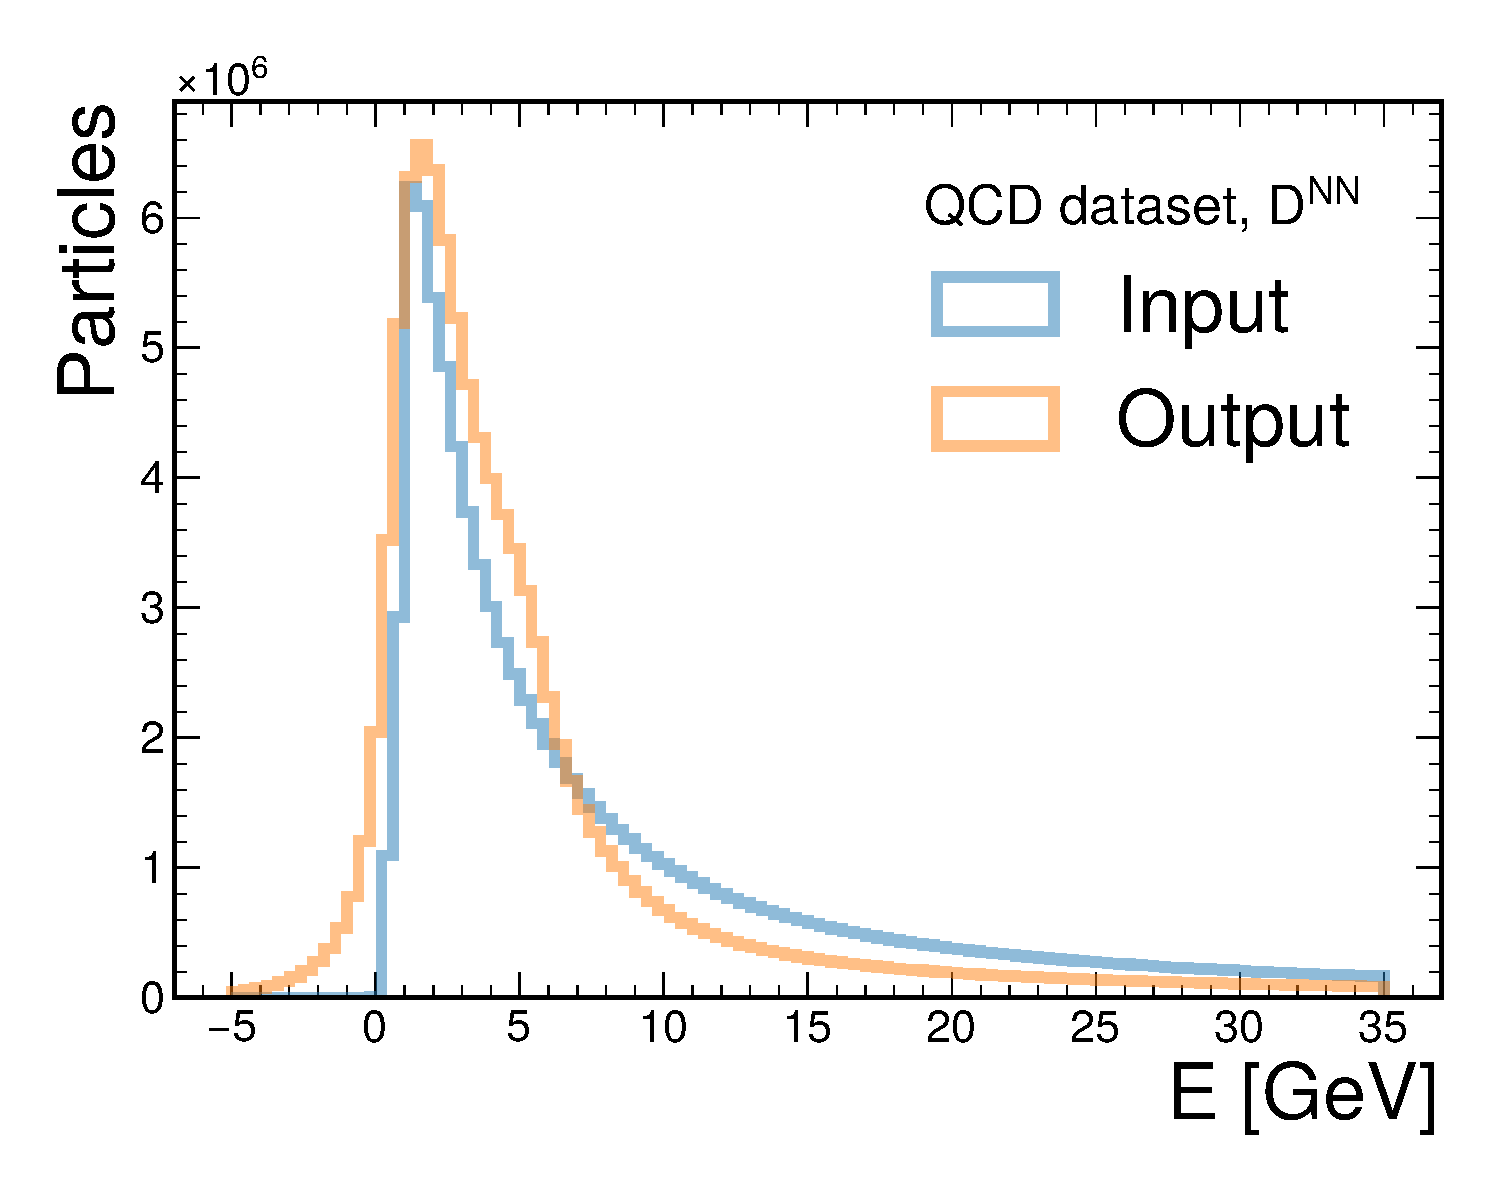
\includegraphics[width=0.24\textwidth]{figures/gae_sparseloss/GNN_AE_EdgeConv_$E$.pdf}
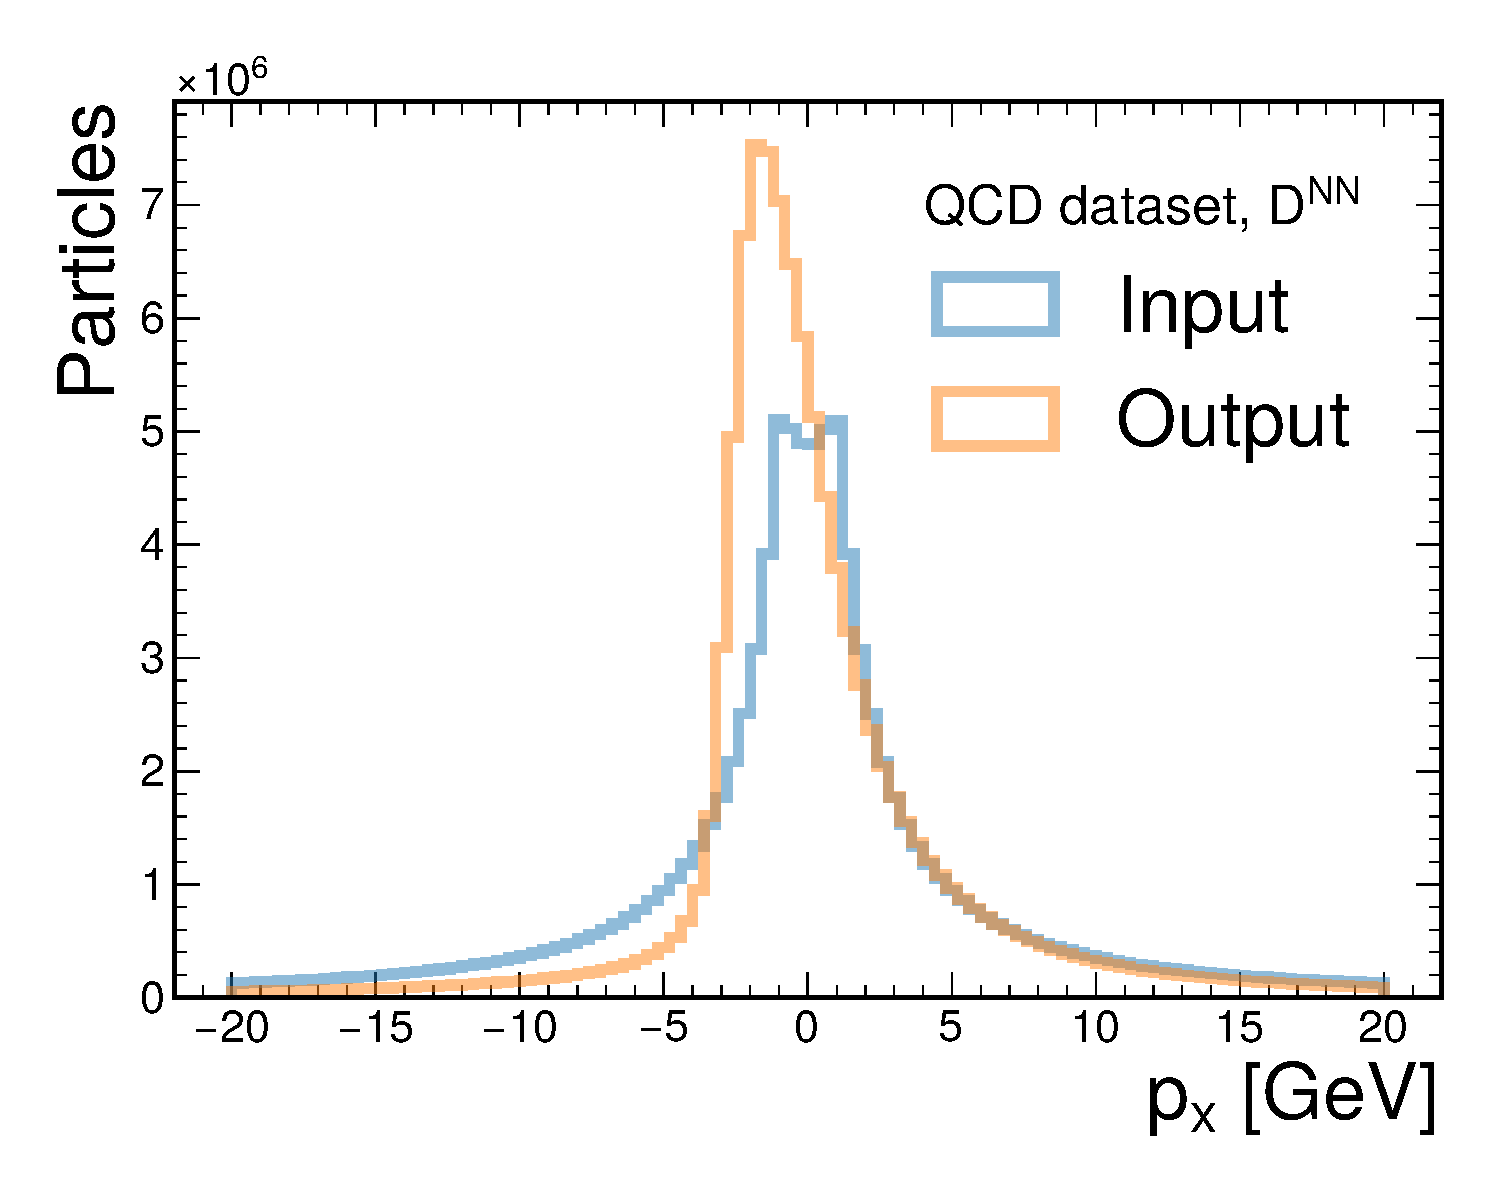
\includegraphics[width=0.24\textwidth]{figures/gae_sparseloss/GNN_AE_EdgeConv_$p_x$.pdf}
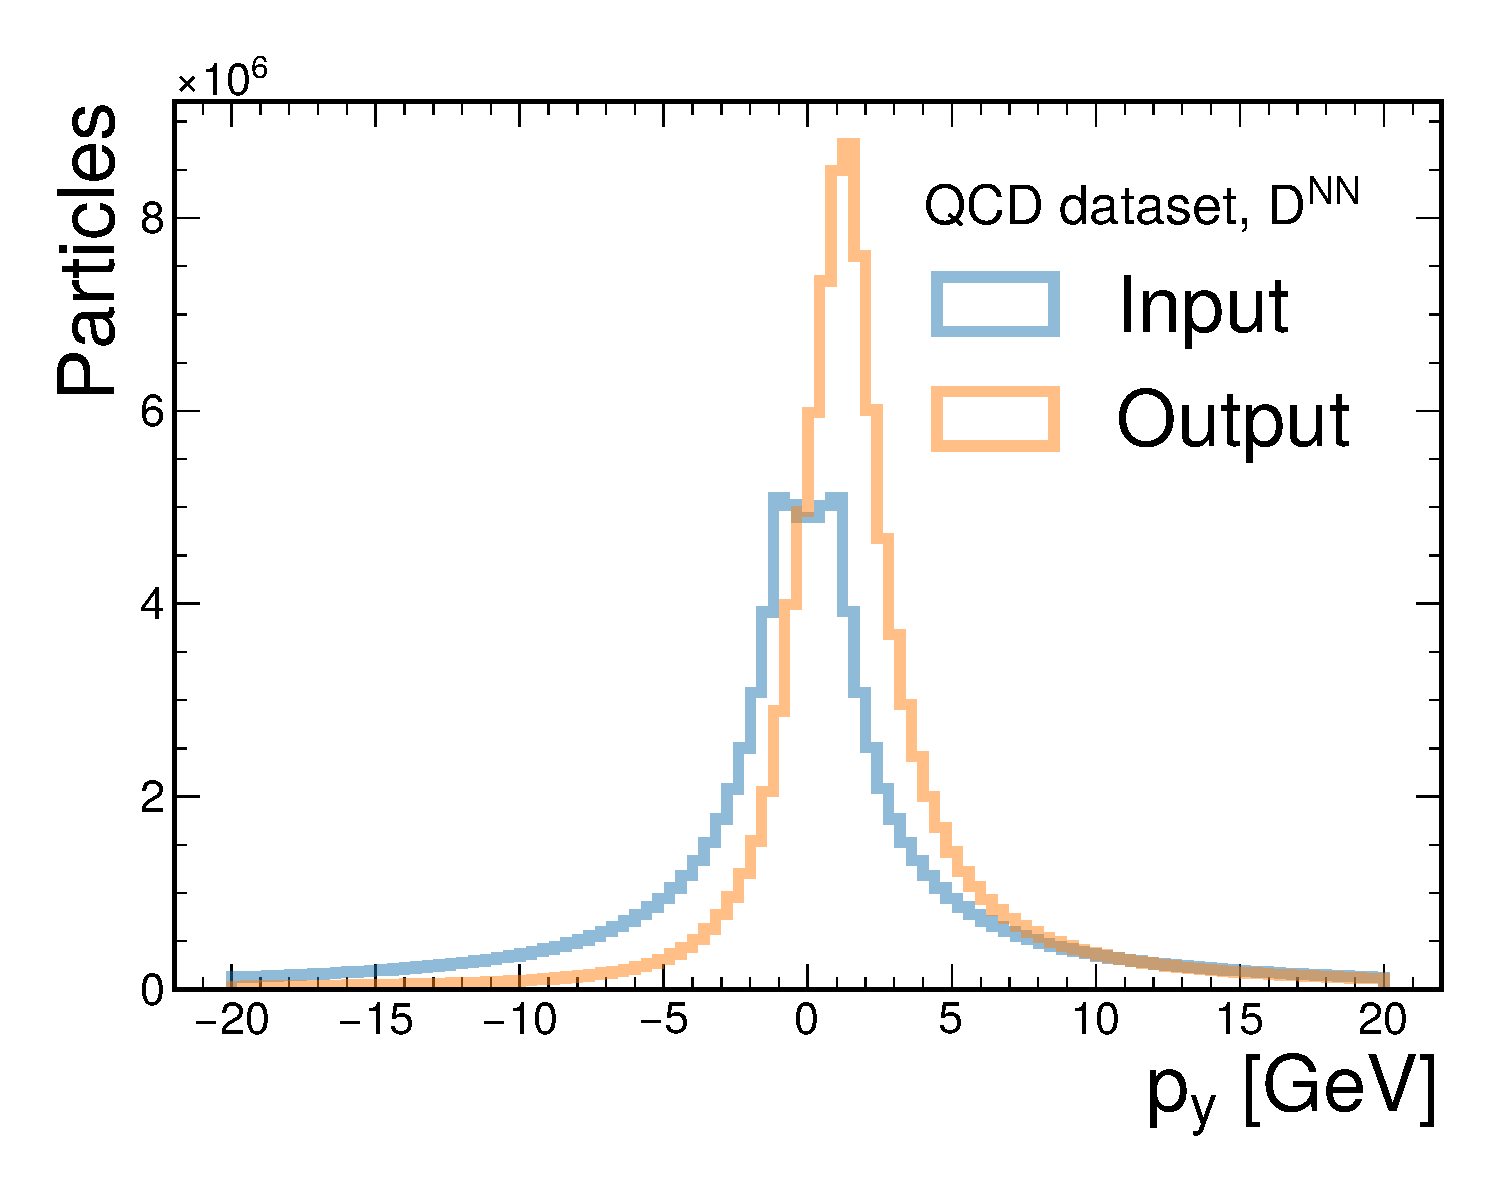
\includegraphics[width=0.24\textwidth]{figures/gae_sparseloss/GNN_AE_EdgeConv_$p_y$.pdf}
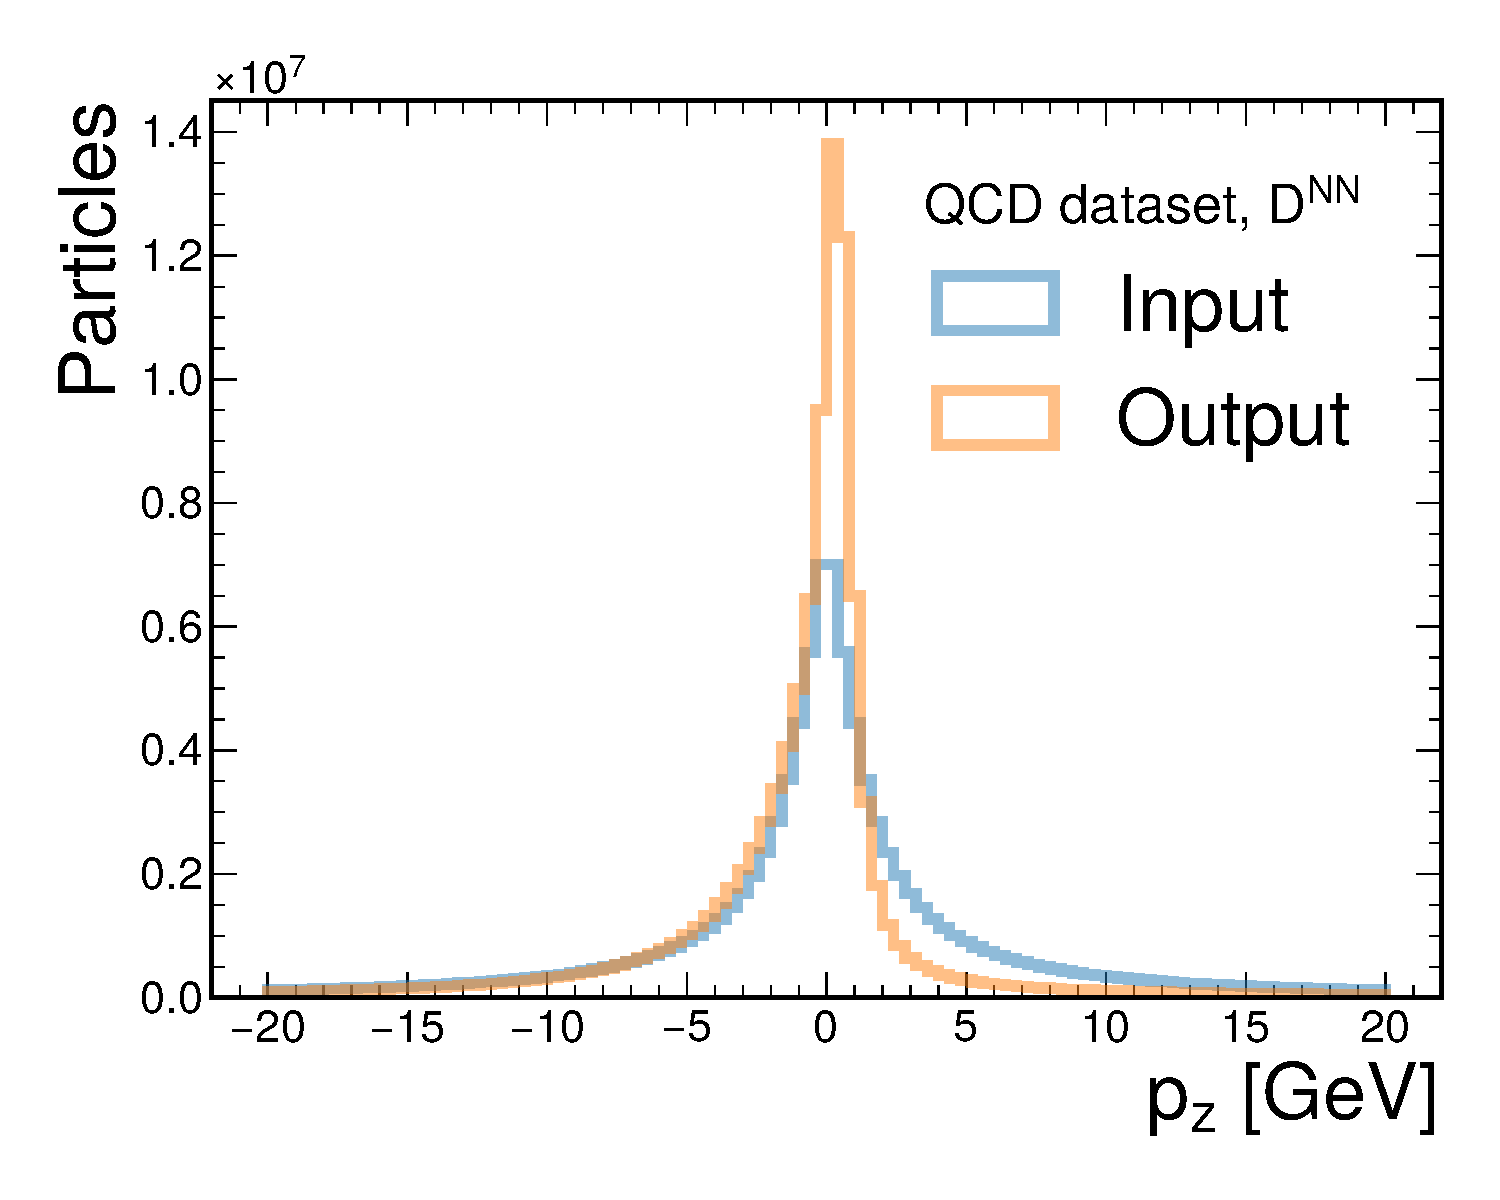
\includegraphics[width=0.24\textwidth]{figures/gae_sparseloss/GNN_AE_EdgeConv_$p_z$.pdf}
\caption{Comparison of input and reconstructed features $E$ (far left), $p_x$ (center left), $p_y$ (center right), and $p_z$ (far right) for the models trained with MSE (top) and $D^\mathrm{NN}$ (bottom) loss functions on the QCD testing dataset.
%The format of the input differs between the two autoencoders, hence differences in the distributions along the same features.
}
\label{fig:reconstruction}
\end{figure}

\subsection{Results on LHC Olympics}

%\noindent \textit{We welcome results on any of the black boxes (BBs) as well as the R\&D dataset.  Please try to minimize any discussion of non-LHCO results.  Figures should be referenced like this: Fig.~\ref{fig:fig1}.}\\

First, we studied our algorithm on the R\&D dataset.
As the truth information is provided, we can create a receiver operating characteristic (ROC) curve to determine the effectiveness of the PGAE to identify a signal ($\PWpr\to\PX\PY$, $\PX\to\Pq\Pq$, and $\PY\to\Pq\Pq$ with $m_{\PWpr} = 3.5$~TeV, $m_\PX = 500$~GeV, and $m_\PY= 100$~GeV) that it did not observe during training.
The ROC curves for both the MSE and $D^\mathrm{NN}$ loss functions are shown in Fig.~\ref{fig:rocs}.
Although the MSE loss is not permutation invariant, we find it provides better discrimination for a new unseen signal.

\begin{figure}
    \centering
    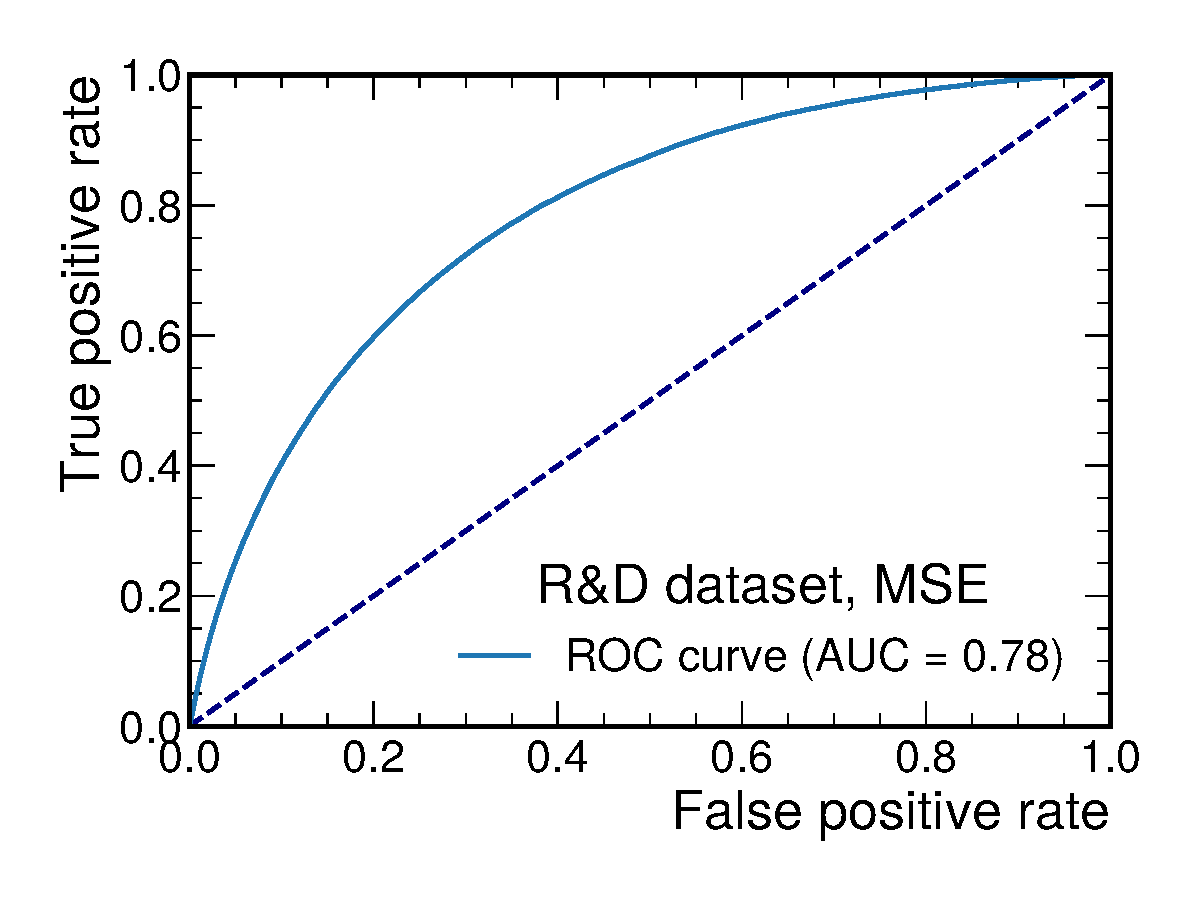
\includegraphics[width=0.45\textwidth]{figures/gae_mse/roc.pdf}
    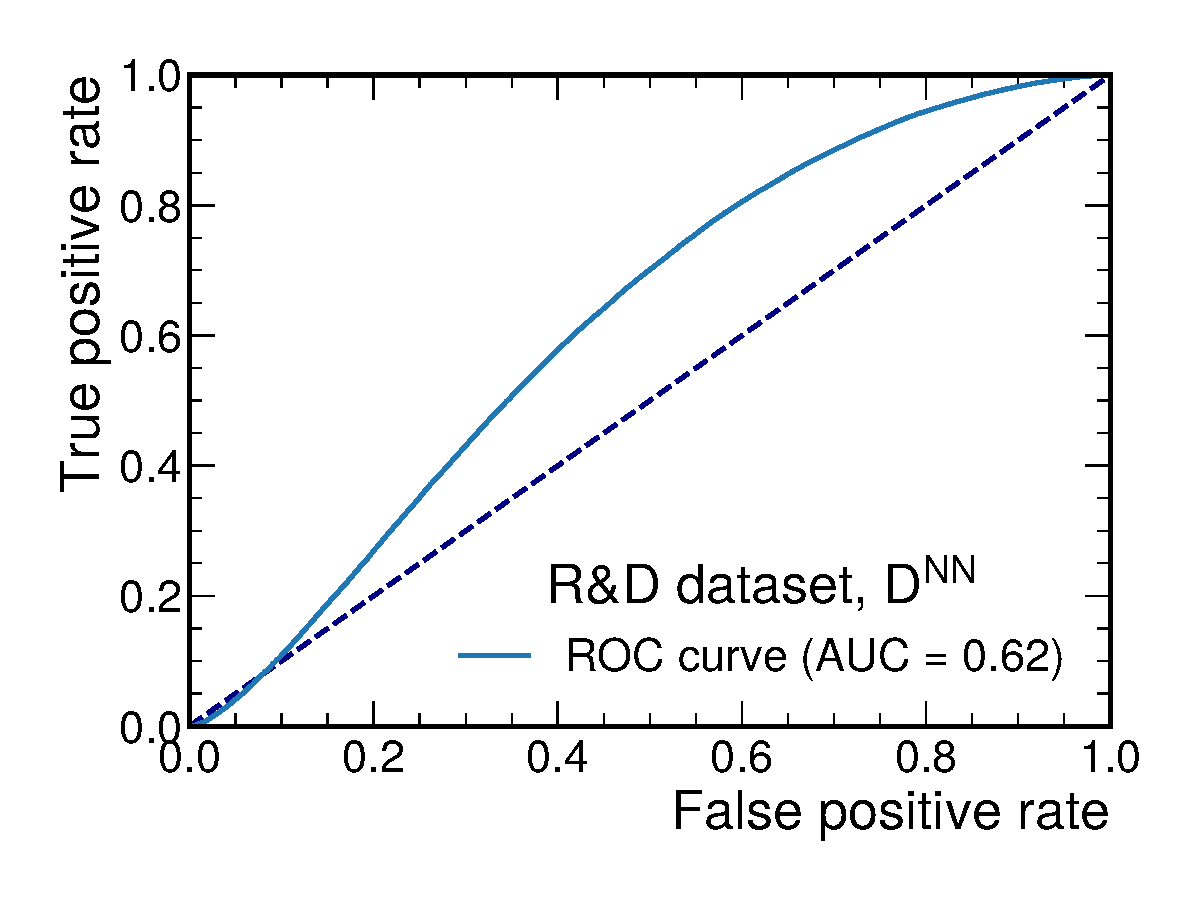
\includegraphics[width=0.45\textwidth]{figures/gae_sparseloss/roc.pdf}
    \caption{ROC curves for the PGAE trained with the MSE (left) and $D^\mathrm{NN}$ loss (right).}
    \label{fig:rocs}
\end{figure}

To evaluate our model's performance for anomaly detection, we perform a resonance search (or ``bump hunt'') in the dijet invariant mass $m_\mathrm{jj}$, computed from the two jets with highest $\pt$ in the event. 
We perform this dijet search in black box (BB) 1, which contains a resonant dijet signal at $m_\mathrm{jj}\sim 3.8$~TeV, and BB 2, which contains no signal.
We require both of the jets to be ``outliers,'' which we define as jets with a reconstruction loss exceeding a threshold corresponding to the 90\% quantile of the loss distribution for the leading two jets in the corresponding evaluation dataset.
We note that because our algorithm is jet-focused, it is straightforward to generalize this search to multijet events.


For the background prediction in the signal-enriched outlier region, we perform a simplified analysis using the shape of the data in the background-enriched nonoutlier region.
Specifically, we fit the ratio of the nonoutlier-to-outlier dijet mass distribution with a fourth-order polynomial to derive a transfer factor (TF).
We take nonoutlier data distribution weighted by the TF as an estimate of the expected background in the outlier region. 
We do not consider systematic uncertainties associated to the TF although these could be taken into account in a more complete analysis in the future.
The procedure is illustrated in Fig.~\ref{fig:fit} for BB 2.

\begin{figure}[htpb]
    \centering
    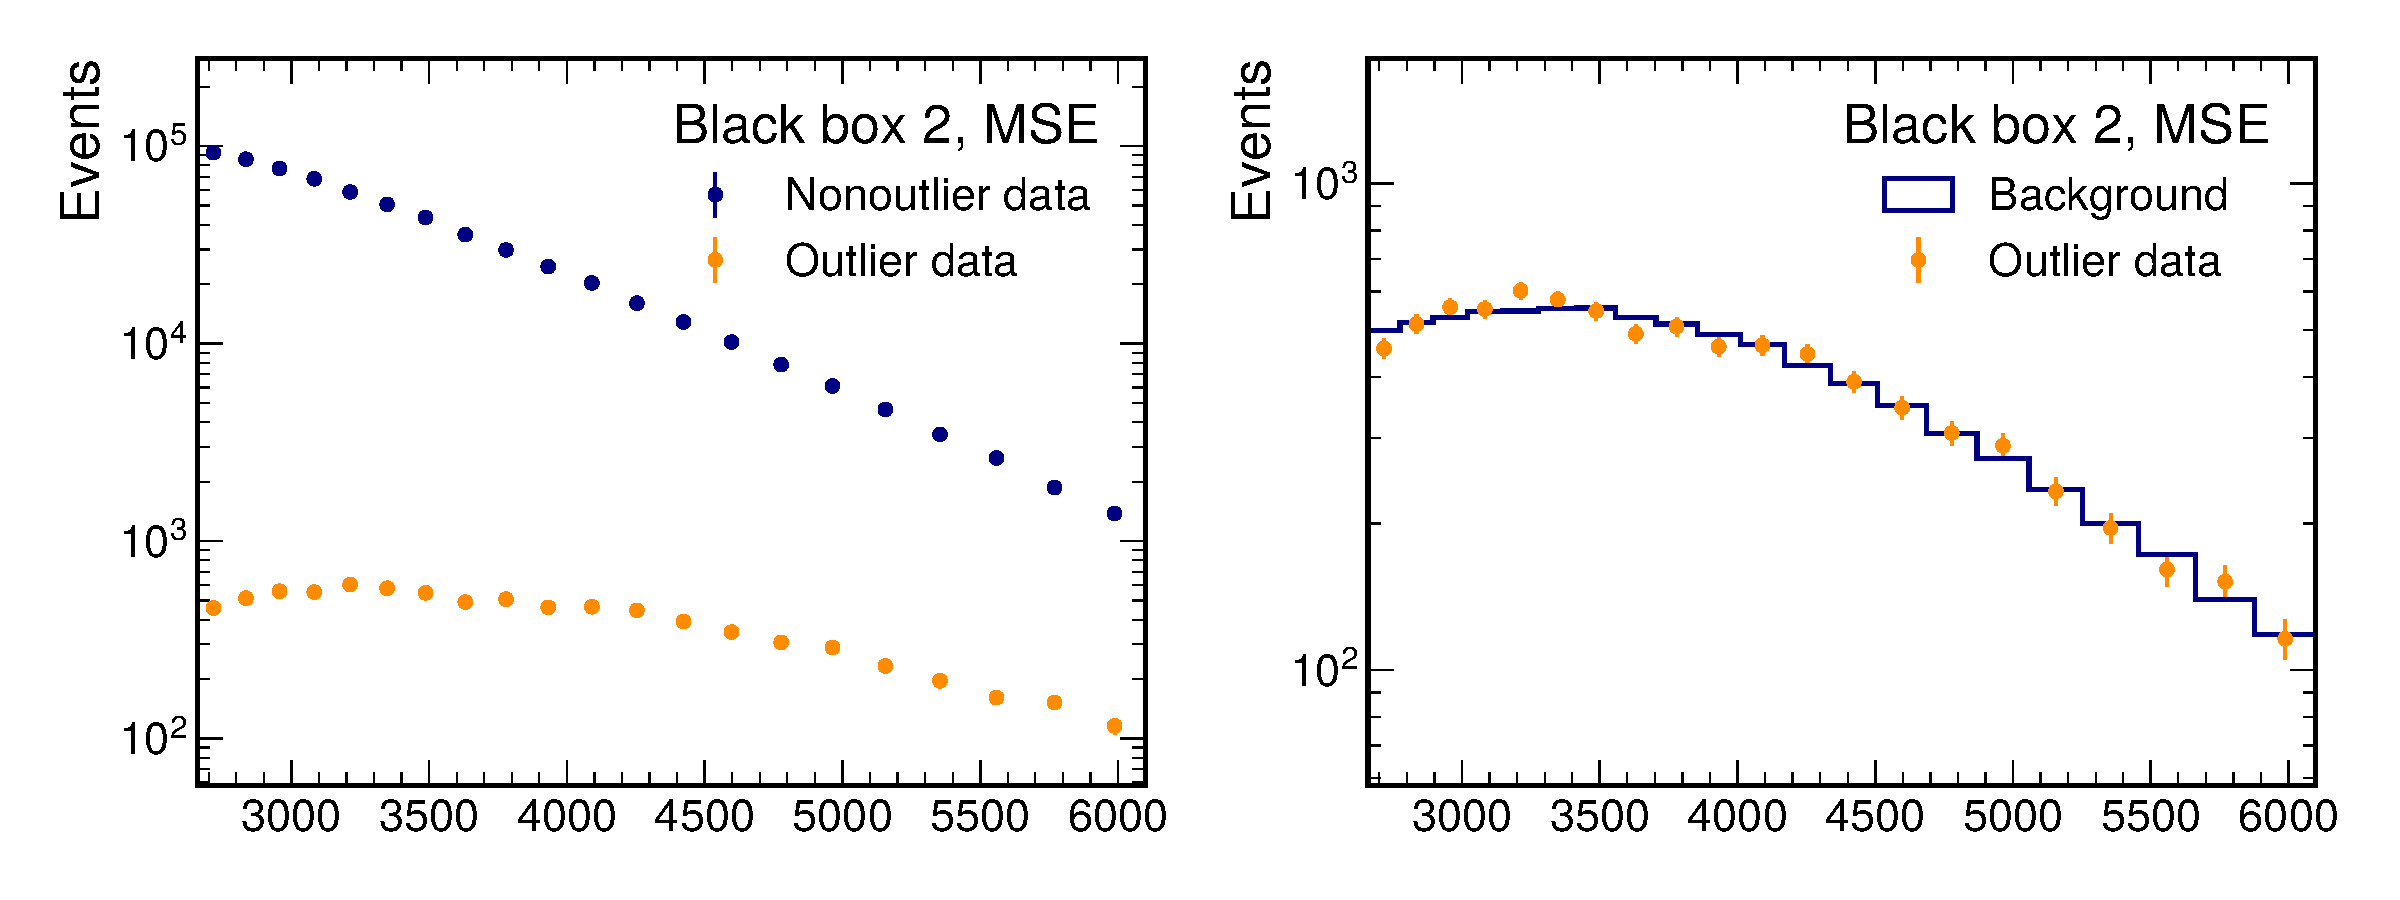
\includegraphics[width=0.9\textwidth]{figures/gae_mse/bb2_GNN_AE_EdgeConv_Finished_fit.pdf}\\
    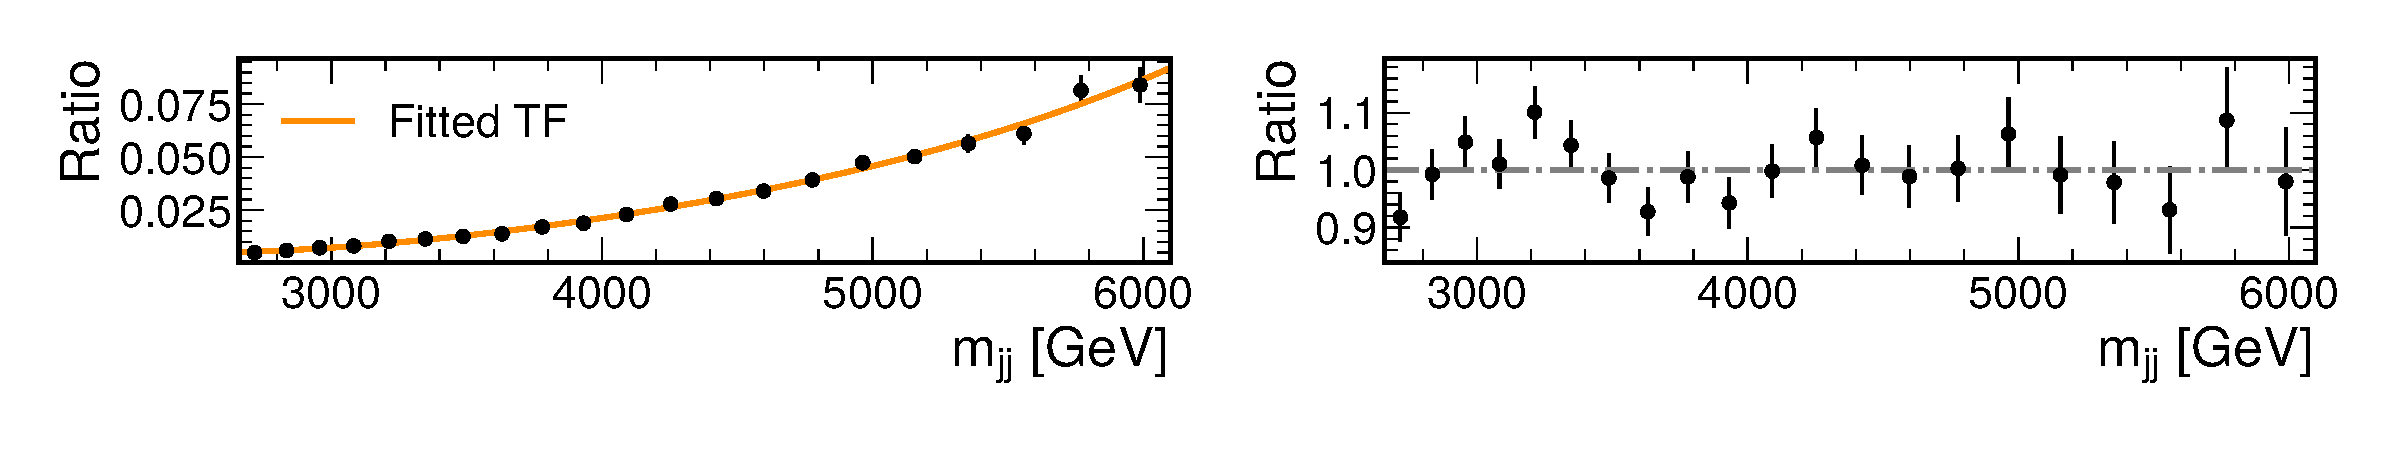
\includegraphics[width=0.9\textwidth]{figures/gae_mse/bb2_GNN_AE_EdgeConv_Finished_fit_ratio.pdf}
    \caption{Illustration of the simplified background estimation procedure in BB 2 for the GAE trained with MSE loss. 
    A comparison between the nonoutlier and outlier jet mass distribution is shown (upper left). 
    The ratio of the two distributions is fit with a fourth-order polynomial to derive a transfer factor (lower left). 
    The corresponding postfit prediction is also shown (upper right). 
    The postfit ratio is randomly scattered around one as expected for BB 2, which contains no signal.}
    \label{fig:fit}
\end{figure}


%%%% update
To derive the observed significance with the simplified background prediction, we use the bump hunter (BH) algorithm~\cite{Choudalakis:2011qn}, recently implemented in Python~\cite{pybumphunter}.
We choose the variable-width mass binning from the CMS dijet searches~\cite{Sirunyan:2018xlo} in the range from 2659~GeV to 6099~GeV.
We look for resonances in windows spanning two to five bins.
With the MSE model in BB 1, we identify a possible resonance around $3.9$~TeV with a local significance of $2.1\,\sigma$, which is close to the region of the injected dijet resonance with $m_\PZpr=3823$~GeV.
In BB 2 using the same model, the most discernable bump lies around $3.3$~TeV with a small local significance of $0.8\,\sigma$, which agrees with the fact that BB 2 has no injected signal. 
For the model trained with the $D^\mathrm{NN}$ loss, a $1.5\,\sigma$ excess is seen at $2.8$~TeV in BB 1 and a $-1.4\,\sigma$ excess at $5.1$~TeV in BB 2. 
Neither is significant.
As noted previously, the permutation invariant $D^\mathrm{NN}$ loss performs worse at the unsupervised anomaly detection task.
This may be due to the minimization, which will often return a smaller loss value than MSE even for poorly reconstructed, anomalous jets.
Fig.~\ref{fig:gnnaebumps} shows the BH results for BBs 1 and 2 using the models trained with both losses.


% bumps...
\begin{figure}[htpb]
    \centering
    \begin{subfigure}[b]{0.45\textwidth}
        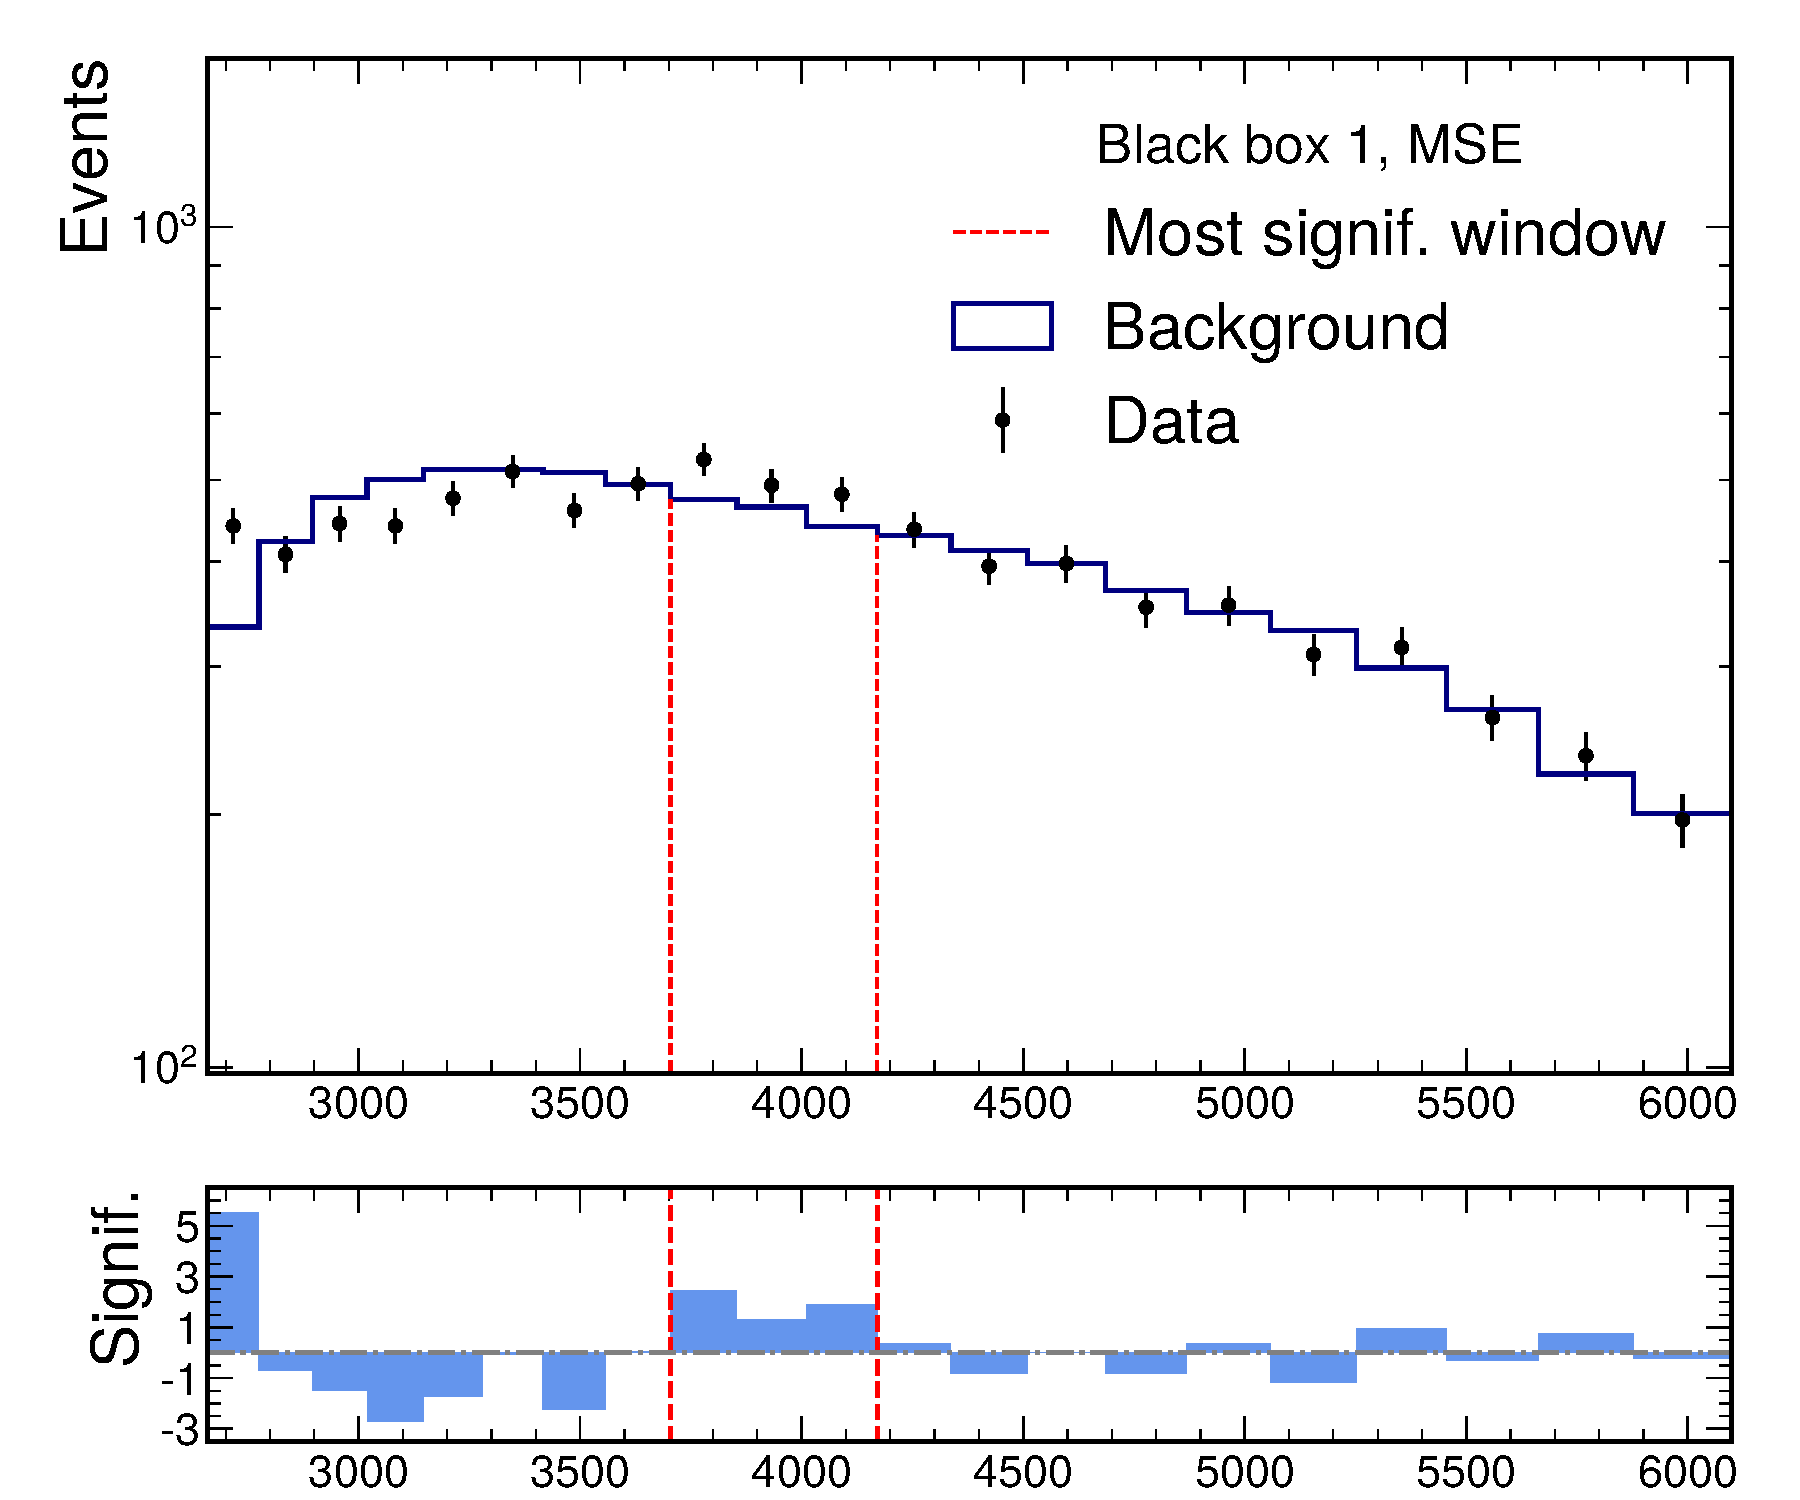
\includegraphics[width=\textwidth]{figures/gae_mse/bb1_GNN_AE_EdgeConv_Finished_bumphunter.pdf}
        \caption*{BB 1, MSE, $2.1\,\sigma$ at $3.9$~TeV}
    \end{subfigure}
    \begin{subfigure}[b]{0.45\textwidth}
        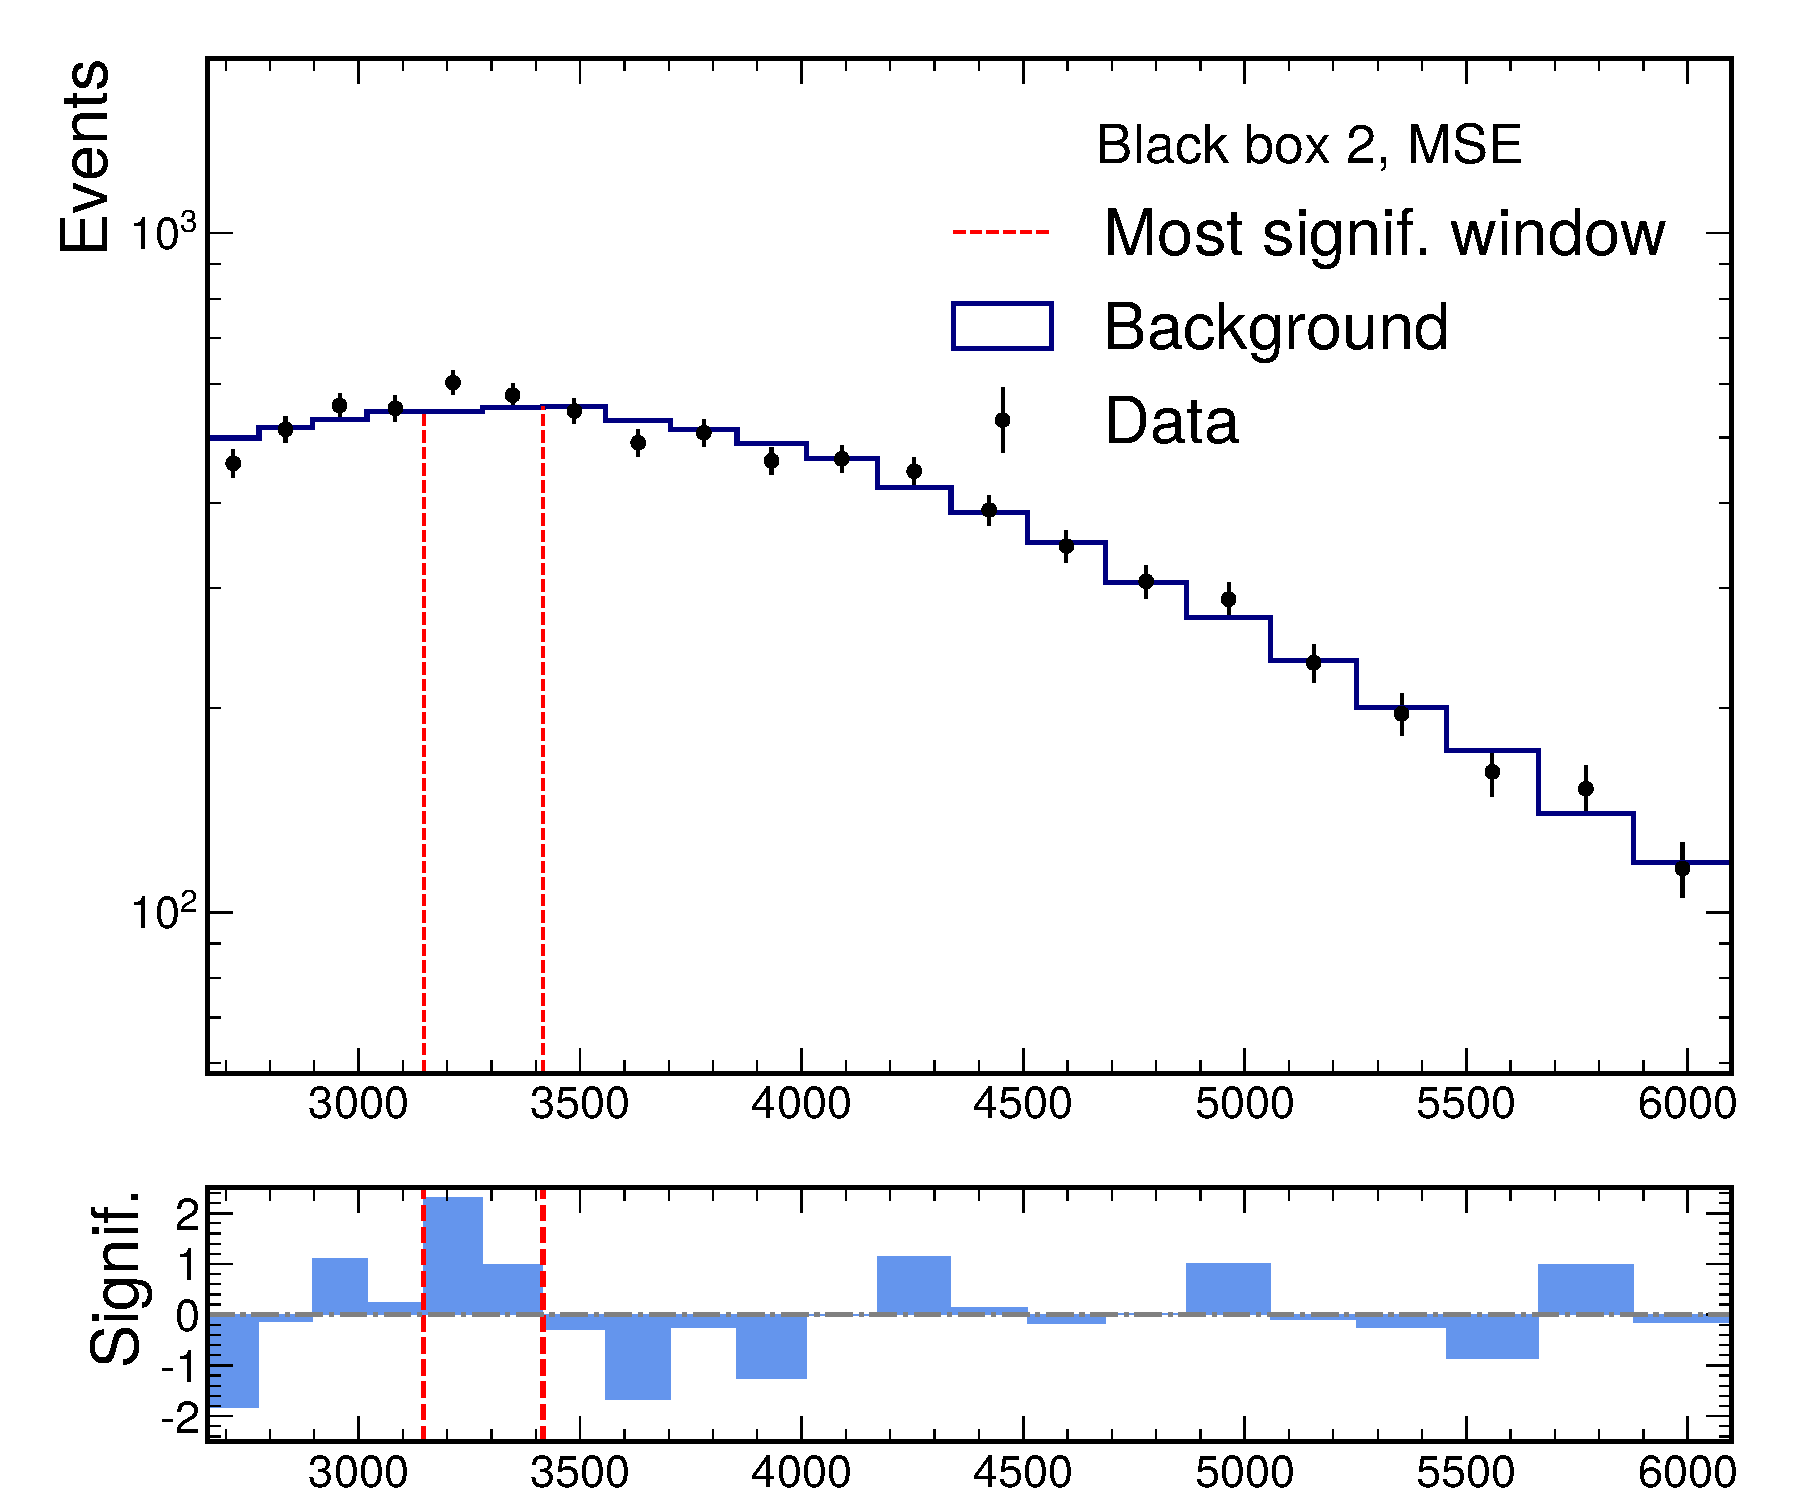
\includegraphics[width=\textwidth]{figures/gae_mse/bb2_GNN_AE_EdgeConv_Finished_bumphunter.pdf}
        \caption*{BB 2, MSE, $0.8\,\sigma$ at $3.3$~TeV}
    \end{subfigure}
    \begin{subfigure}[b]{0.45\textwidth}
        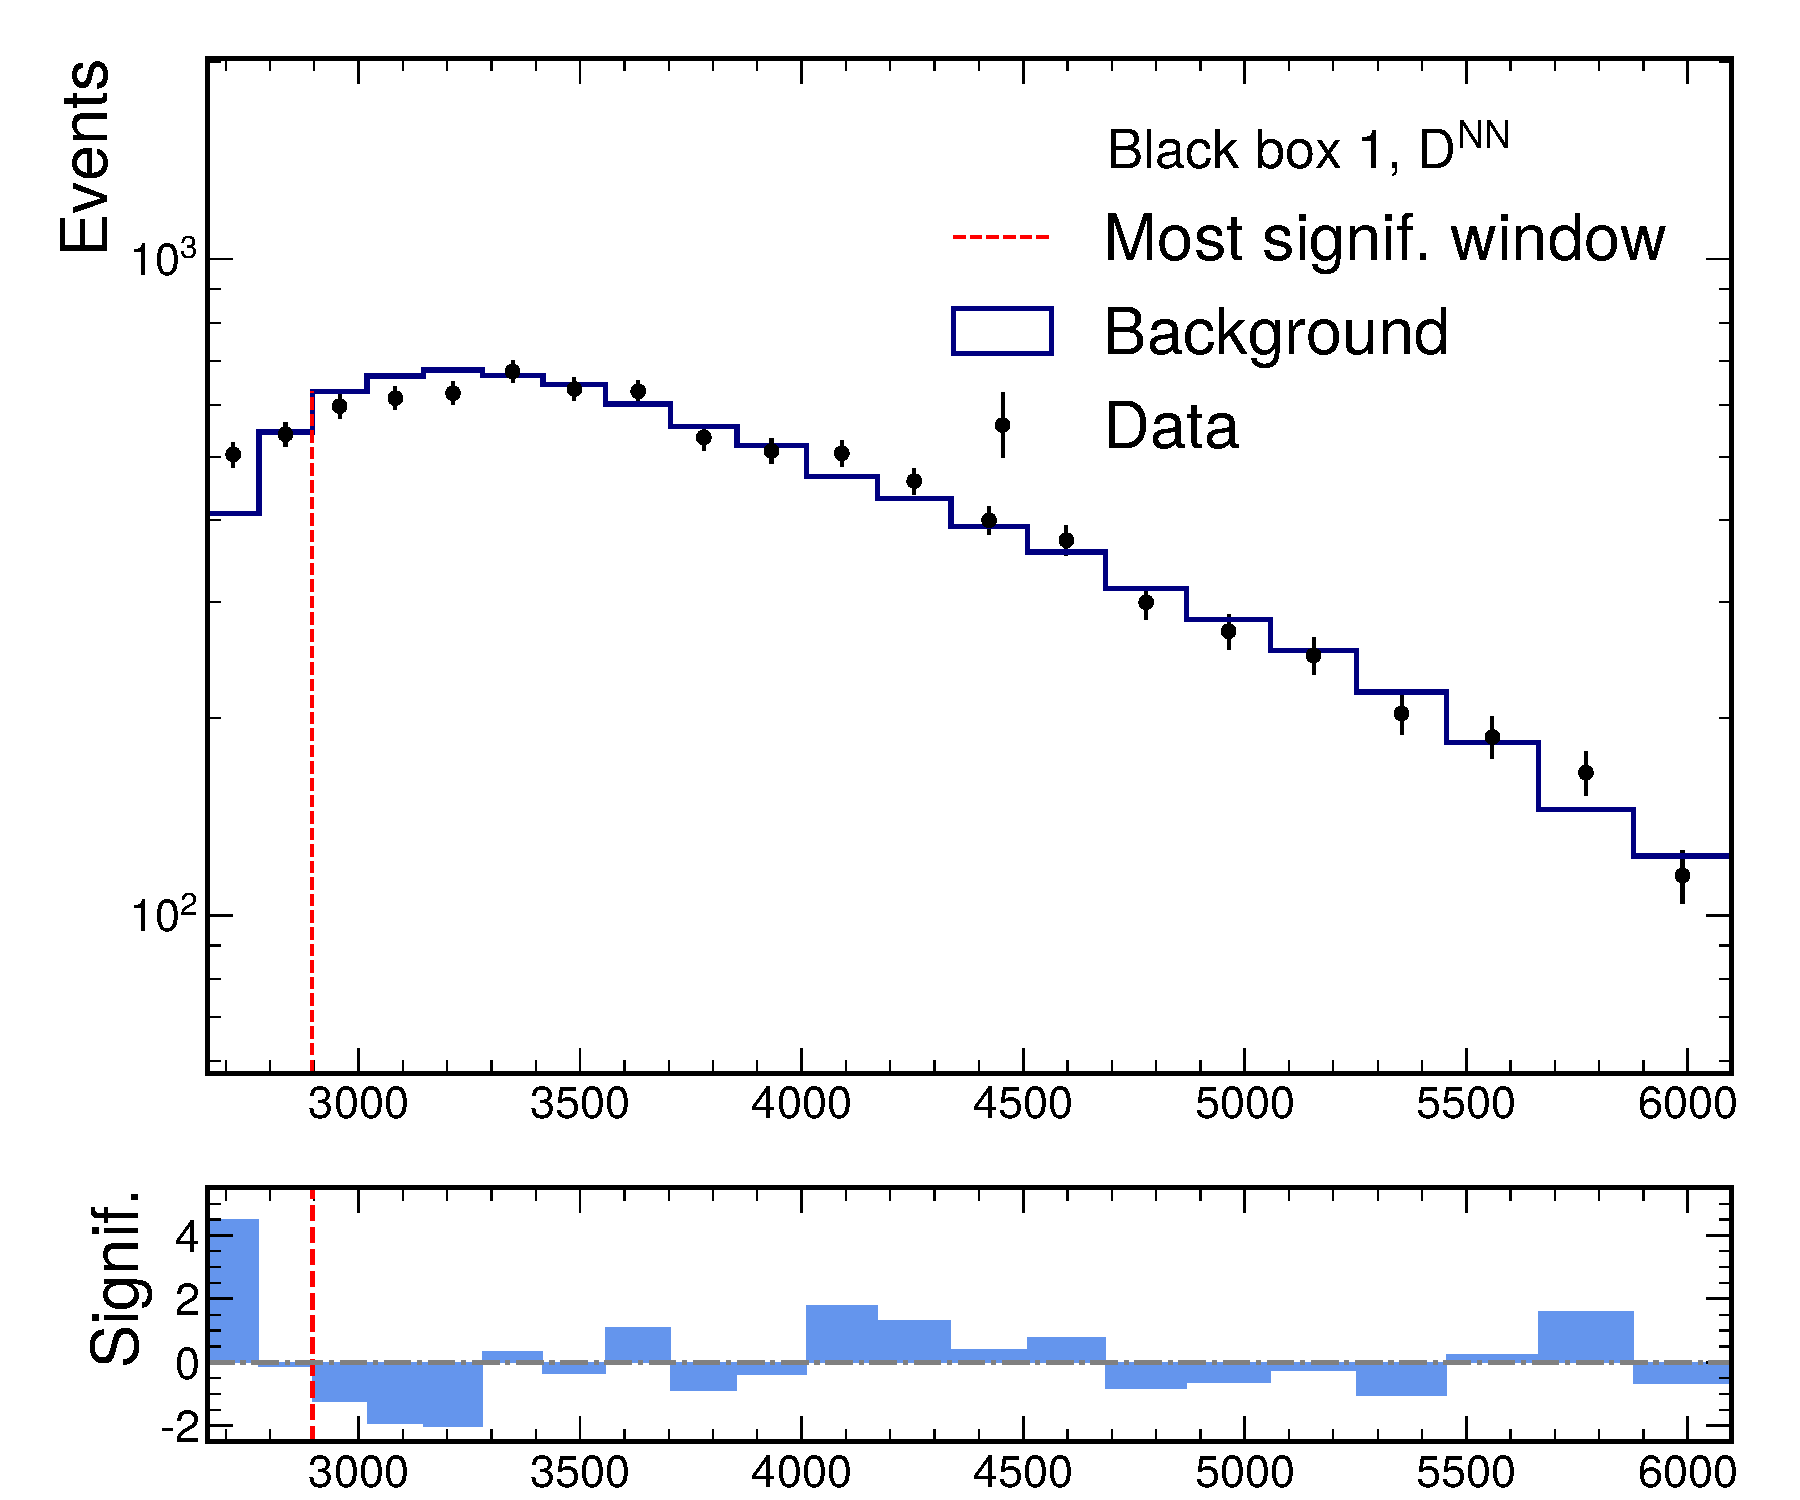
\includegraphics[width=\textwidth]{figures/gae_sparseloss/bb1_EdgeNetSparseLoss_bumphunter.pdf}
        \caption*{BB 1, $D^\mathrm{NN}$, $1.5\,\sigma$ at $2.8$~TeV}
    \end{subfigure}
    \begin{subfigure}[b]{0.45\textwidth}
        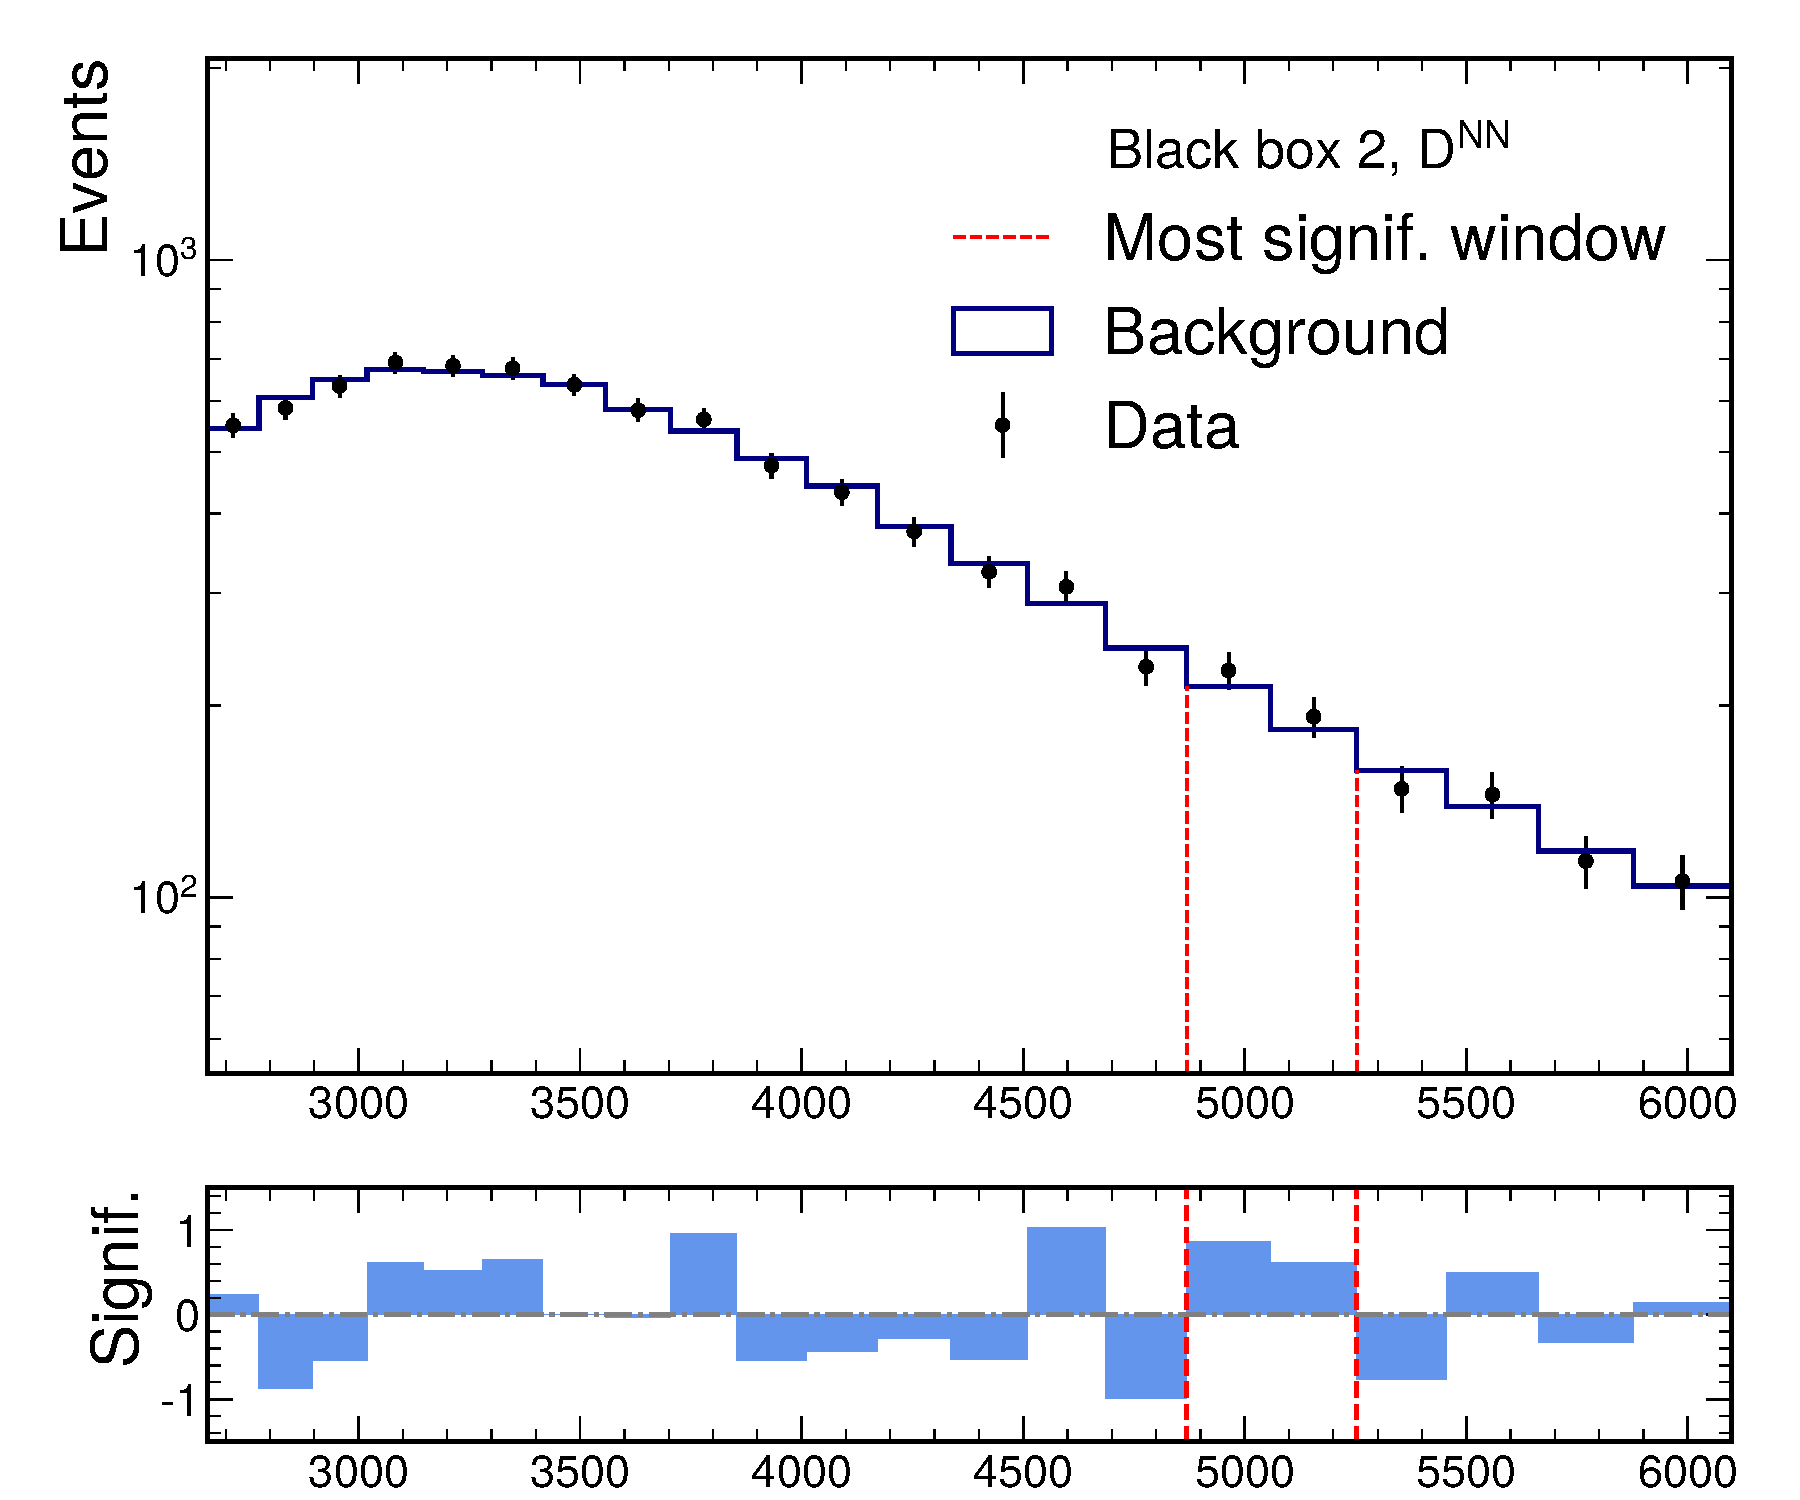
\includegraphics[width=\textwidth]{figures/gae_sparseloss/bb2_EdgeNetSparseLoss_bumphunter.pdf}
        \caption*{BB 2, $D^\mathrm{NN}$, $-1.4\,\sigma$ at $5.1$~TeV}
    \end{subfigure}
\caption{Bump hunt in the dijet invariant mass in BB 1 (left) and 2 (right) using MSE (top) and $D^\mathrm{NN}$ (bottom) as the loss functions.
Outlier jets have a reconstruction loss in the top 10\% with respect to the corresponding BB. 
Outlier events are required to have both jets be outliers.
BB 1 has an anomalous large-radius dijet signal $\PZpr \to \PX\PY \to (\Pq\Pq)(\Pq\Pq)$ injected at $m_\PZpr=3823$~GeV (with $m_\PX = 732$~GeV and $m_\PY= 378$~GeV), while BB 2 has no injected anomalies.
}
\label{fig:gnnaebumps}
\end{figure}


%%%% old
%DELETE: When performing a bump hunt in $m_\mathrm{jj}$ as seen in Fig.~\ref{fig:gnnaebumps}, we fail to discern any noticeable bumps in black box 1 or 2 using the MSE model. 
%Using the nearest neighbor distance loss, in black box 1 we see a potentially significant bump at approximately $3.8$~TeV, which encapsulates the region of the injected dijet resonance anomaly at $m_\PZpr=3823$~GeV.  
%In contrast, for the $m_\mathrm{jj}$ bump hunt in black box 2, which has no injected anomalies, we do not observe any significant bumps.

\subsection{Lessons Learned}
\label{sec:lessons}

%\noindent \textit{Please say anything that you learned from the experience in general, what you learned specifically from the results, what you improved after you learned about BB1, what you would change in the future, etc.}
Graph neural networks, like our proposed particle graph autoencoder, are promising methods for anomaly detection.
However, further work is needed to define a permutation-invariant loss function for use with such architectures that is more performant for anomaly detection.
In addition, a more generic resonance search procedure, such a multimensional fit in the trijet, dijet, trijet, and single-jet mass distributions possibly using methods like Gaussian process fitting~\cite{Frate:2017mai}, would be appropriate to use in combination with this algorithm.
In our experience, the R\&D dataset was extremely helpful in preparing our anomaly detection algorithms and gauging whether the algorithm we were developing was on the right track. 
In the future, more extensive R\&D datasets, together with additional black boxes with different signals, may be useful.
Finally, it may be productive to host a future competition on a well-known platform, such as Kaggle, to increase engagement with the broader machine learning community.

\subsection{Code Availability}
\label{code:code}

All code is publicly available at \url{https://github.com/stsan9/AnomalyDetection4Jets}.

%%%%%%%%%%%%%%%%%%%%%%%%
\acknowledgments

We thank the University of California San Diego Triton Research and Experiential
Learning Scholars (TRELS) program for supporting this research.
We also thank Joosep Pata for helpful discussions.
J.~D. is supported by the U.S. Department of Energy (DOE), Office of Science, Office of High Energy Physics Early Career Research program under Award No. DE-SC0021187.
M.~P. is supported by the European Research Council (ERC) under the European Union's Horizon 2020 research and innovation program (Grant Agreement No. 772369).
J-R.~V. is partially supported by the European Research Council (ERC) under the European Union's Horizon 2020 research and innovation program (Grant Agreement No. 772369) and by the U.S. DOE, Office of Science, Office of High Energy Physics under Award No. DE-SC0011925, DE-SC0019227, and DE-AC02-07CH11359.
This work was supported in part by U.S. National Science Foundation (NSF) awards CNS-1730158, ACI-1540112, ACI-1541349, OAC-1826967, the University of California Office of the President, and the University of California San Diego's California Institute for Telecommunications and Information Technology/Qualcomm Institute. 
Thanks to CENIC for the 100~Gpbs networks.

\vspace{10mm}


\bibliographystyle{jhep}
\bibliography{HEPML}
\end{document}
